\chapter{Economia de Energia, Controle da Latência e Otimização de Desempenho}

Este capítulo apresenta os resultados quantitativos obtidos através de nossas simulações em busca de uma economia de energia ainda maior, e do aumento de performance em relação ao \emph{Energy Efficient Ethernet} padrão. Para isso, combinamos primeiramente o EEE com \emph{Packet Coalescing}, maximizando assim a economia de energia, em seguida, utilizamos dois diferentes AQMs, o \emph{Random Early Detection} e o \emph{Controlled Delay}, juntamente com \emph{Explicit Congestion Notification} para diminuir a latência e aumentar a performance nas cargas de trabalho do \emph{Hadoop 3.x MapReduce}.

Redes de \emph{data centers} estão começando a empregar uma nova geração de \emph{switches} com \emph{buffers} maiores, para acomodar comunicações em rajadas (\emph{bursty}) e oferecer melhor desempenho nas aplicações. Uma grande parte dos aplicativos atualmente usa o TCP como protocolo de transmissão, e sofrem com grande latência de pacotes, devido à tendência do TCP de utilizar totalmente o buffer disponível. \emph{Switches} recentes que implementam AQM e suportam ECN permanecem com estas tecnologias desativadas, deixando desnecessariamente um recurso que poderia reduzir significativamente diminuir a latência melhorando assim a performance \cite{silva2018eon}.

Com este estudo, encontramos economias de energia ideais para as conexões acima de 10GbE, mas somente quando o \emph{Packet Coalescing} está habilitado. Com o \emph{Packet Coalescing}, os \emph{switches} atrasam intencionalmente os pacotes de saída enquanto o link está no modo LPI, para que possam ser transmitidos consecutivamente com os pacotes subsequentes \cite{silva2018eon}. As configurações do \emph{Packet Coalescing}, no entanto, devem ser cuidadosamente escolhidas e testadas para evitar uma perda excessiva de desempenho.

\section{Energy Efficient Ethernet com Packet Coalescing}

A metodologia de forma detalhada está presente no Capítulo 3. Para o EEE, primeiramente testamos o modo \emph{Deep Sleep}, e posteriormente o \emph{Fast Wake}. Quanto ao \emph{Packet Coalescing}, assumimos valores de configurações de 12$\mu$s10 e 120$\mu$s100 \cite{christensen2010ieee}, 500$\mu$s500 \cite{silva2018eon} e 1ms1000 \cite{reviriego2010burst}.

\subsection{Economia de Energia}

Durante nossos experimentos não encontramos economia de energia suficiente para conexões de 1GbE que justificasse a implementação do \emph{Packet Coalescing}, pelo contrário, em alguns casos ainda houve um aumento do gasto energético em 0.17\% (de 0.0805 w/h para 0.0810 w/h), como no caso dos \emph{Batch Jobs} em topologia 4:1.

Para conexões de 10GbE, o gasto energético foi reduzido de 18.32\% (0.4909 w/h) para 11.82\% (0.3168 w/h) com a configuração 120$\mu$s100, reduzindo assim quase pela metade do consumo de energia em relação ao EEE padrão. Para este link a pior configuração foi de 12$\mu$s10, o que resultou em uma redução baixa do consumo de 18.32\% para 15.08\% (0.4042 w/h), seguida de e 1ms1000 com redução de 18.32\% para 15.06\% (0.4035 w/h).

Em links de 25GbE, a redução foi ainda mais significativa, caindo de 19.82\% (1.0725 w/h) para 13.37\% (0.7235 w/h) na configuração 120$\mu$s100. Neste link, a pior economia foi obtida pela configuração 1ms1000, que reduziu o consumo de 19.82\% para 16.71\% (0.904 w/h). Uma redução do consumo de 19.86\% (1.4877 w/h) para 13.24\% (0.9917 w/h) foi encontrada em conexões de 40GbE com o EEE no modo \emph{Deep Sleep} ao aplicar a configuração 120$\mu$s100, fazendo com que este link obtivesse um gasto energético similar ao de 25GbE.

Para as conexões de 100GbE com o EEE no modo \emph{Deep Sleep}, a redução do consumo foi de 24.31\% (2.6469 w/h) para 15.72\% (1.7115 w/h) em nossa melhor configuração 120$\mu$s100, e 19.29\% (2.1010 w/h) em nossa pior 12$\mu$s10.

A maior redução do consumo de energia foi encontrada em conexões de 400GbE ao aplicarmos o \emph{Packet Coalescing} com a configuração 120$\mu$s100, reduzindo assim o consumo do EEE em relação ao Ethernet Padrão de 48.11\% (10.6853 w/h) para 25.88\% (5.7483 w/h). Neste link, a pior configuração foi de 12$\mu$s10, o que resultou em uma redução de 48.11\% para 30.67\% (6.8107 w/h).

\begin{figure}[!htb]
    \centering
    \label{fig:EEEDeepSleepPaCo}
    
    \subfloat[\centering Consumo de energia do EEE no modo \emph{Deep Sleep} com \emph{Packet Coalescing} em conexões de 1GbE \label{fig:EEEDeepSleepPaCo1GbE}]{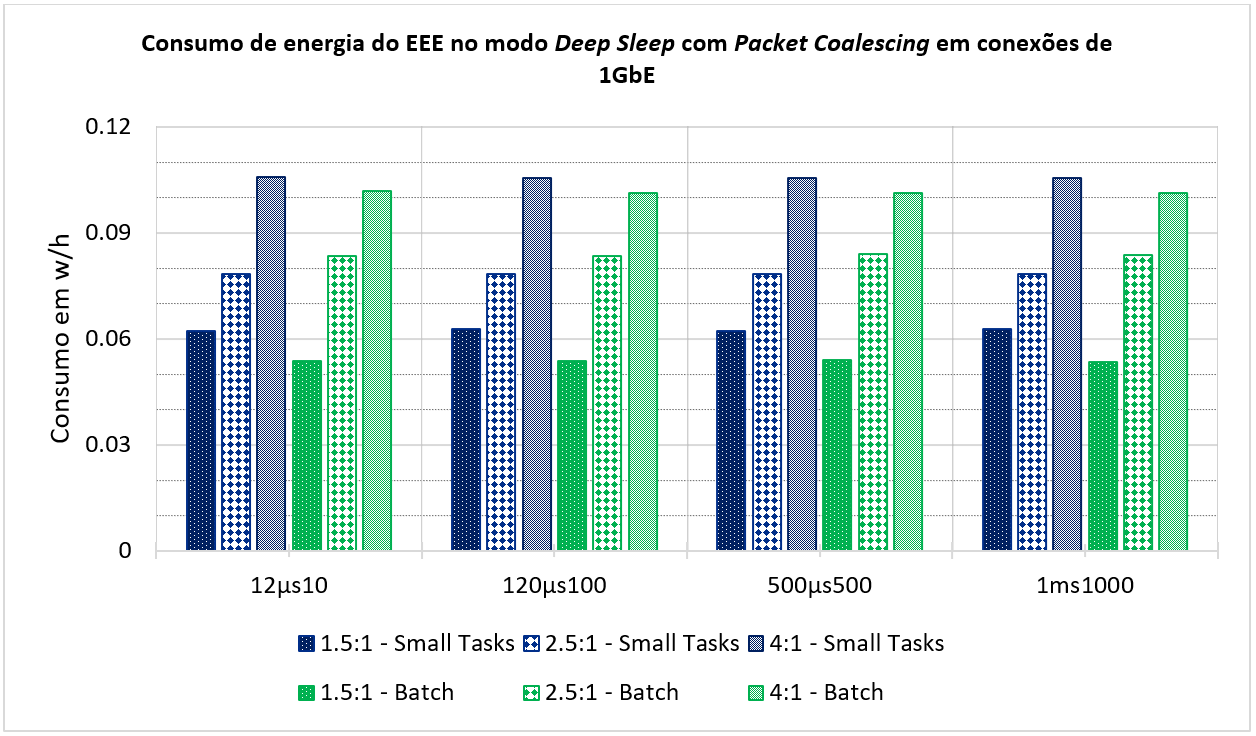
\includegraphics[width=8cm]{5-EEECoDelHadoop/EEEDeepSleepPaco_1GbE.PNG}}\hfill
    \subfloat[\centering Consumo de energia do EEE no modo \emph{Deep Sleep} com \emph{Packet Coalescing} em conexões de 10GbE
    \label{fig:EEEDeepSleepPaCo10GbE}]{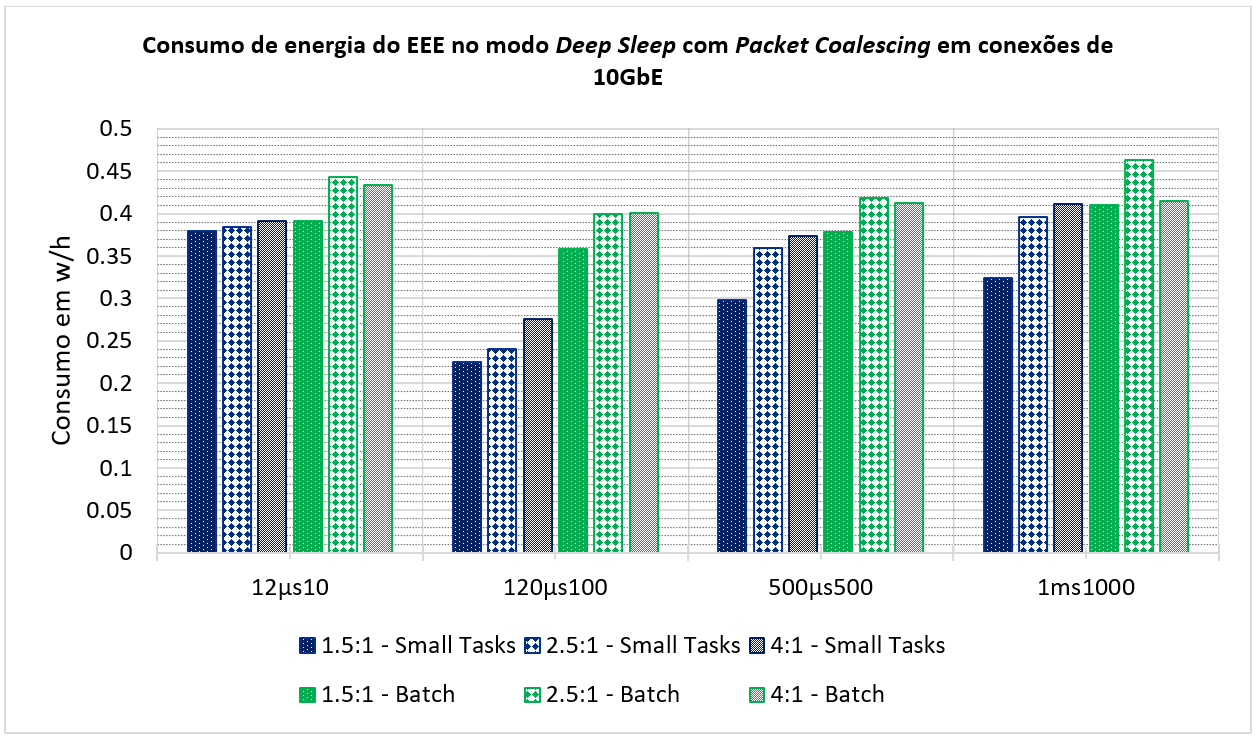
\includegraphics[width=8cm]{5-EEECoDelHadoop/EEEDeepSleepPaco_10GbE.PNG}}
    
    \subfloat[\centering Consumo de energia do EEE no modo \emph{Deep Sleep} com \emph{Packet Coalescing} em conexões de 25GbE \label{fig:EEEDeepSleepPaCo25GbE}]{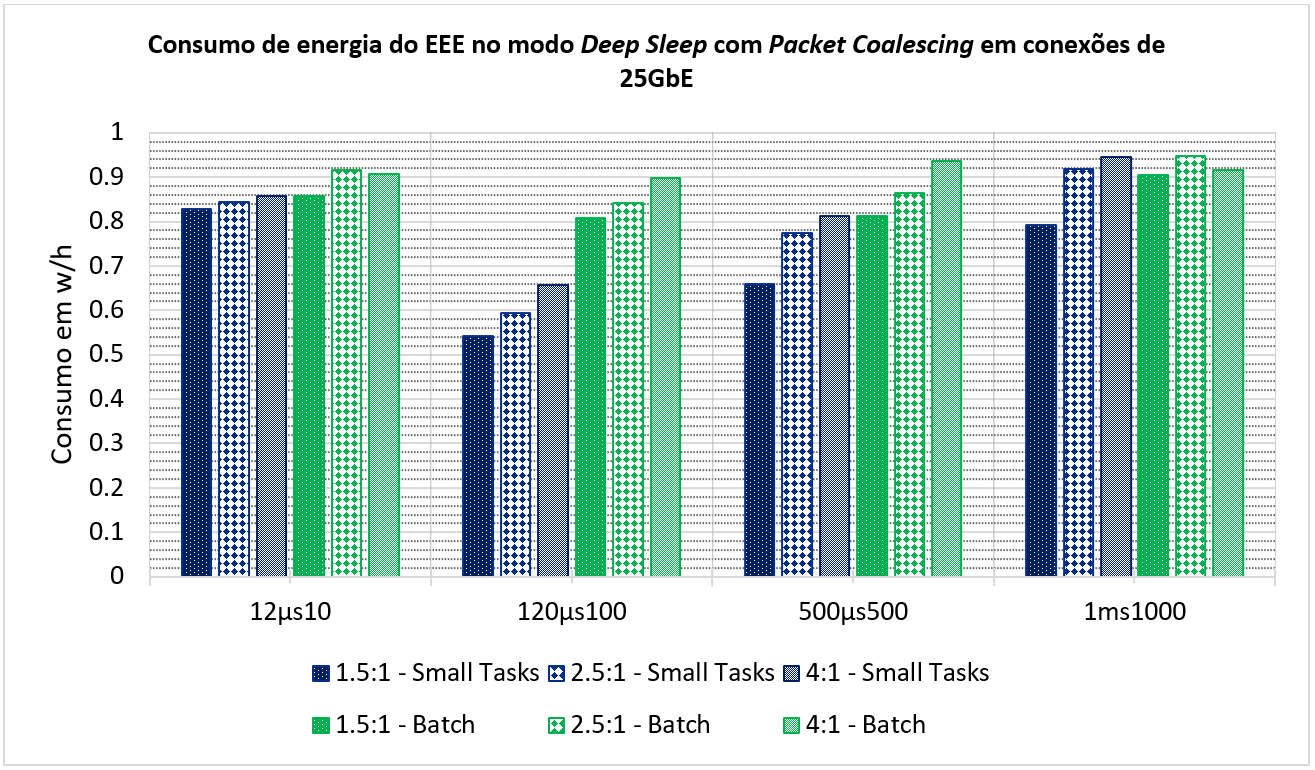
\includegraphics[width=8cm]{5-EEECoDelHadoop/EEEDeepSleepPaco_25GbE.PNG}}\hfill
    \subfloat[\centering Consumo de energia do EEE no modo \emph{Deep Sleep} com \emph{Packet Coalescing} em conexões de 40GbE
    \label{fig:EEEDeepSleepPaCo40GbE}]{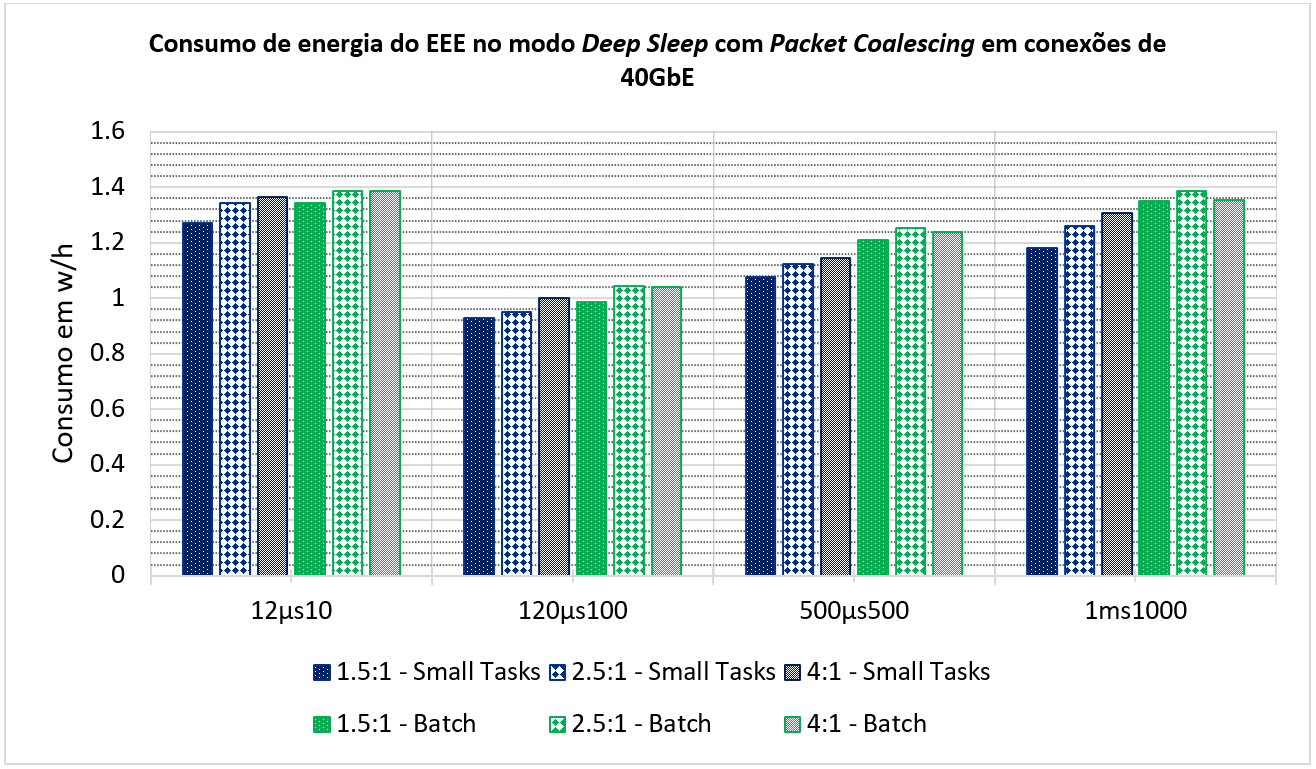
\includegraphics[width=8cm]{5-EEECoDelHadoop/EEEDeepSleepPaco_40GbE.PNG}}    
    
    \subfloat[\centering Consumo de energia do EEE no modo \emph{Deep Sleep} com \emph{Packet Coalescing} em conexões de 100GbE
    \label{fig:EEEDeepSleepPaCo100GbE}]{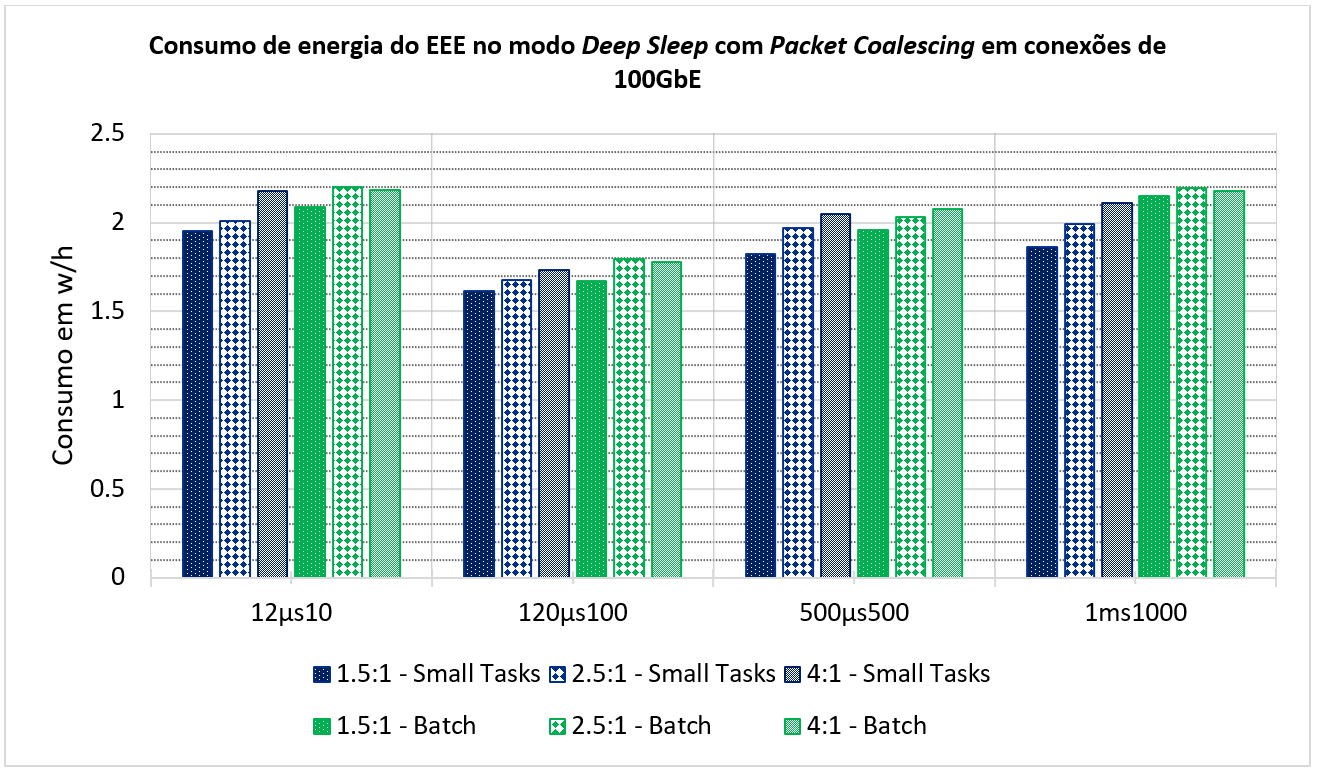
\includegraphics[width=8cm]{5-EEECoDelHadoop/EEEDeepSleepPaco_100GbE.PNG}}\hfill
    \subfloat[\centering Consumo de energia do EEE no modo \emph{Deep Sleep} com \emph{Packet Coalescing} em conexões de 400GbE
    \label{fig:EEEDeepSleepPaCo400GbE}]{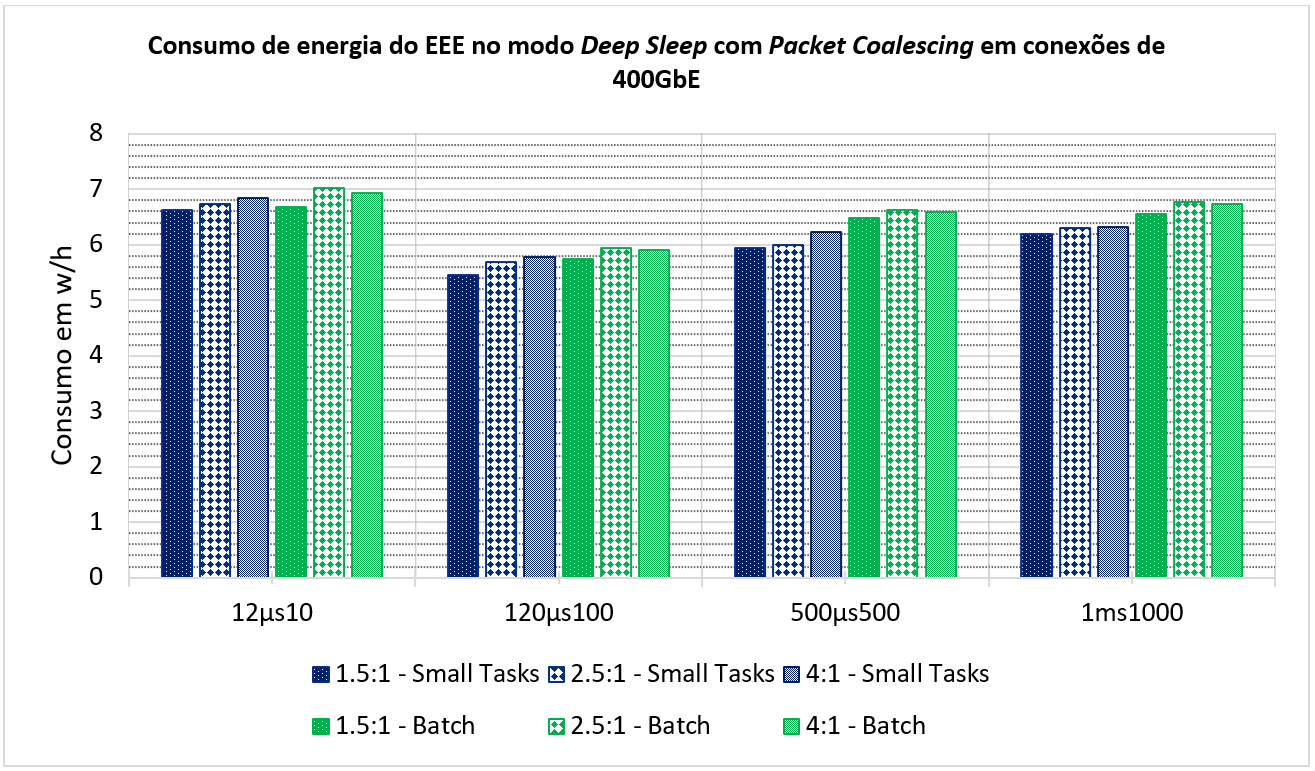
\includegraphics[width=8cm]{5-EEECoDelHadoop/EEEDeepSleepPaco_400GbE.PNG}}       
    
    \caption{\centering Consumo de energia do EEE no modo \emph{Deep Sleep} com \emph{Packet Coalescing}}
\end{figure}

O modo \emph{Fast Wake} do EEE tende a consumir mais energia que o modo padrão, \emph{Deep Sleep}.  Para este modo também encontramos reduções no consumo de energia consideráveis nos links que abrigam esta tecnologia no momento, 40GbE e 100GbE.  No caso dos links de 40GbE o gasto energético em relação ao Ethernet foi reduzido de 61.87\% (4.6340 w/h) para 40,3\% (3.0182 w/h) em nossa melhor configuração 120$\mu$s100, e de 61.87\% para 54.83\% (4.1067 w/h) na pior 12$\mu$s10. Para os links de 400GbE nossa melhor configuração do \emph{Packet Coalescing} 120$\mu$s100, reduziu o consumo de  63.51\% (6.9160 w/h) para 40.37\% (4.3966 w/h).

As figuras 5.1 e 5.2 ilustram todos os resultados expostos nesta subseção, e revelam ainda que \emph{Batch Jobs} tendem a gastar em média 1\% de energia a mais que os \emph{Small Tasks}, e em ambos, pode-se reduzir o consumo de energia através de uma taxa de assinatura excessiva baixa (próxima à 1:1).

\begin{figure}[!htb]
    \centering
    \label{fig:EEEFastWakePaCo}
    
    \subfloat[\centering Consumo de energia do EEE no modo \emph{Fast Wake} com \emph{Packet Coalescing} em conexões de 40GbE
    \label{fig:EEEFastWakePaCo40GbE}]{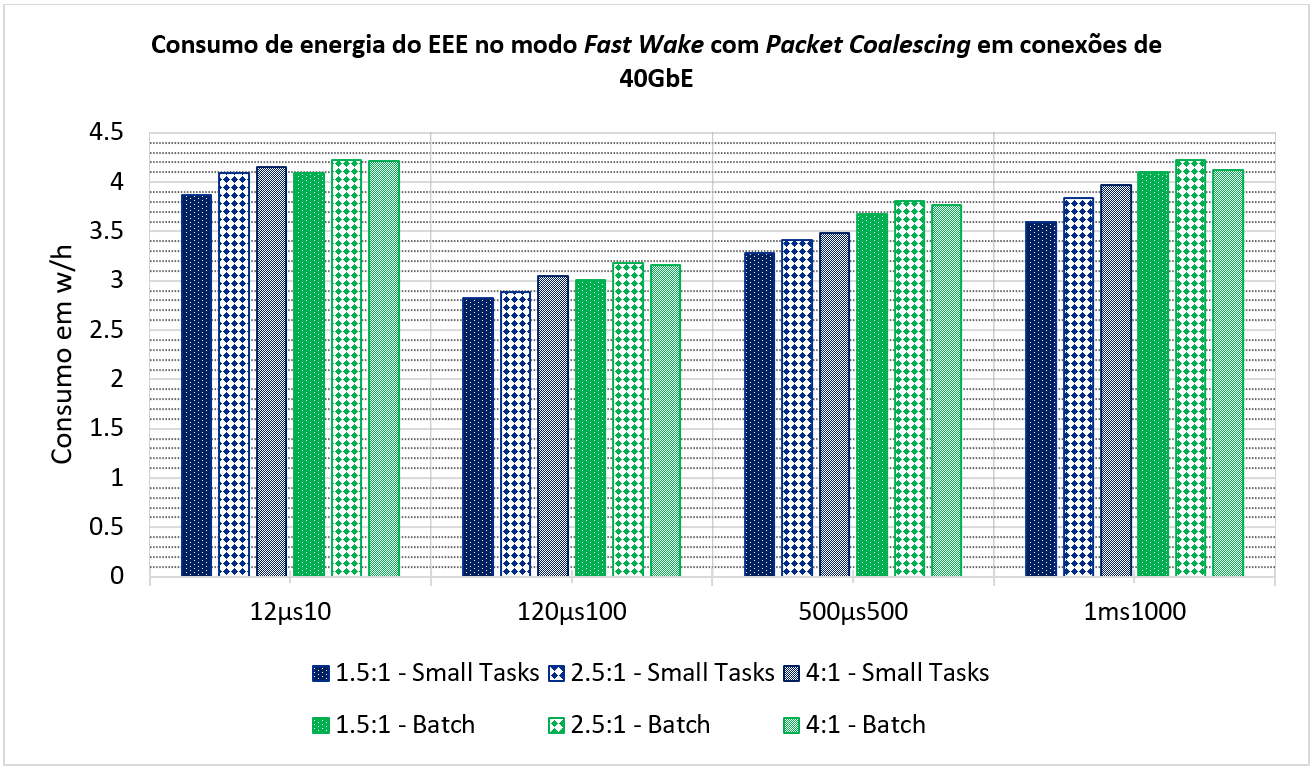
\includegraphics[width=8cm]{5-EEECoDelHadoop/EEEFastWakePaco_40GbE.PNG}}\hfill
    \subfloat[\centering Consumo de energia do EEE no modo \emph{Fast Wake} com \emph{Packet Coalescing} em conexões de 100GbE
    \label{fig:EEEFastWakePaCo100GbE}]{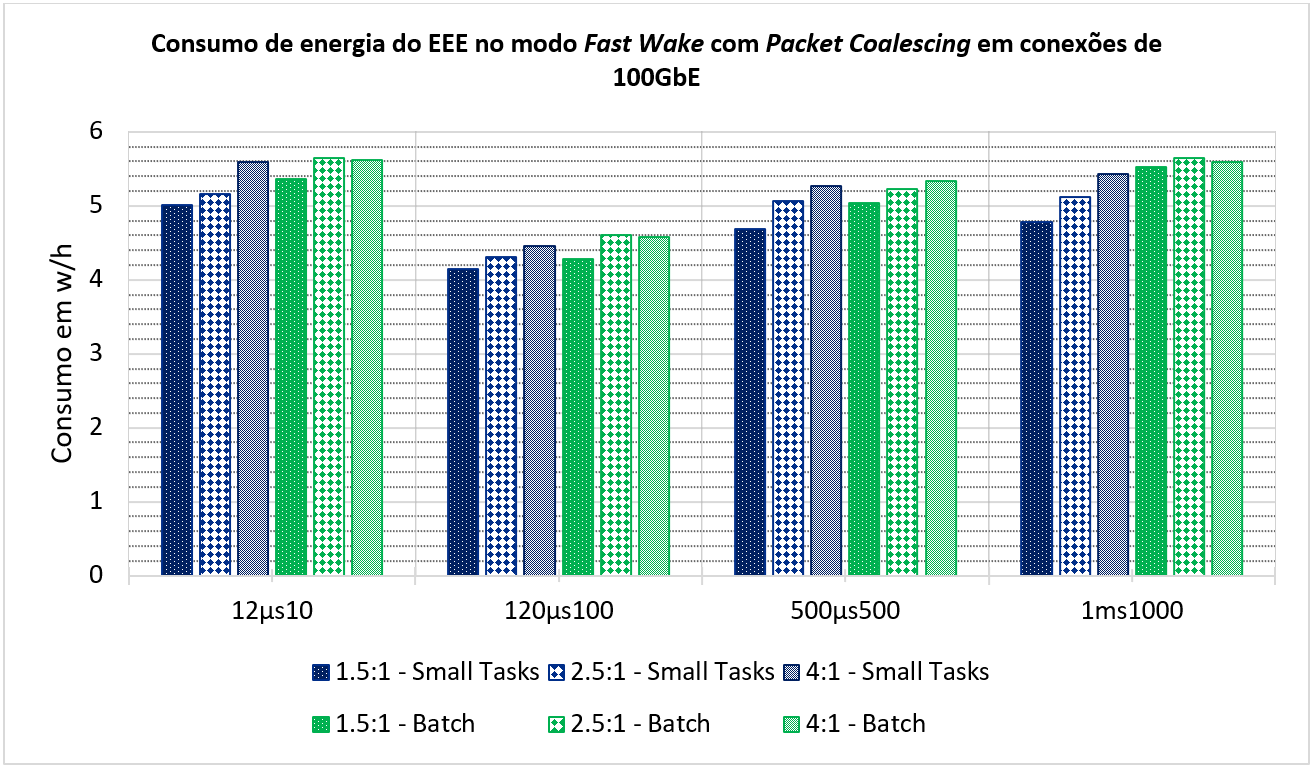
\includegraphics[width=8cm]{5-EEECoDelHadoop/EEEFastWakePaco_100GbE.PNG}}
    
    \caption{\centering Consumo de energia do EEE no modo \emph{Fast Wake} com \emph{Packet Coalescing}}
\end{figure}

\subsection{Desempenho}

Como observado por \cite{mostowfi2011saving} e \cite{silva2018eon}, aplicar o \emph{Packet Coalescing} em conexões com \emph{Energy Efficient Ethernet} sem estar configurado corretamente pode acarretar em uma degradação do desempenho do \emph{Cluster}, além de não obter uma economia de energia vantajosa. Nesta subseção estão expostos os resultados de performance das nossas simulações, em que identificamos configurações que à mantém relativamente estável, enquanto outras a degradam exponencialmente.

As figuras 5.3 e 5.4 ilustram os resultados para o \emph{Packet Coalescing} combinado com EEE no modo \emph{Deep Sleep} e \emph{Fast Wake} respectivamente. Em conexões de 1GbE a melhor configuração 12$\mu$s10 trouxe uma ligeira melhora no desempenho, de 99.783\% para 99.92\% em relação ao Ethernet padrão. Por outro lado, uma configuração ruim como é o caso de 1ms1000, degradou o desempenho para 52.566\%.

Os links de 10GbE demonstraram performance relativamente iguais quando configurados com 12$\mu$s10 e 120$\mu$s100, cera de 99.175\% e 99.141\%. Por outro lado, a configuração de 1ms1000 degradou o desempenho para 52.352\%. Nos links de 25GbE e 40GbE, as configurações 12$\mu$s10 e 120$\mu$s100 também surgiram efeitos parecidos, melhorando levemente o desempenho de 98.472\% para 98.53\% e de 97.147\% para 98.26\%. Assim como nas conexões anteriores, a configuração 1ms1000 degradou o desempenho para 51.577\% e 50.189\%.

A partir das conexões de 100GbE, o desempenho da configuração 12$\mu$s10 degradou-se em relação à 120$\mu$s100. No caso dos links de 100GbE, obtivemos uma estabilidade do desempenho ao utilizarmos 120$\mu$s100, passando de 95.44\% para 95.53\%, enquanto 12$\mu$s10 reduziu o desempenho para 93.13\%. Para 400GbE, 120$\mu$s100 alterou o desempenho de 91.41\% para 91.51\%, enquanto 12$\mu$s10 o reduziu para 87.476\%.

Em todos os casos a configuração 1ms1000 degradou o desempenho em mais de 40\%. Isso se deve ao fato de que configurar o \emph{Packet Coalescing} com tempos de espera e gatilhos maiores fazem com que a rede tenha transmissões mais intensas (\emph{burstiness}), o que pode causar perda de pacotes Ethernet \cite{mostowfi2011saving} e \cite{silva2018eon}.

\begin{figure}[!htb]
    \centering
    \label{fig:PerfEEEDeepSleepPaCo}
    
    \subfloat[\centering Desempenho do EEE no modo \emph{Deep Sleep} com \emph{Packet Coalescing} em relação ao Ethernet Padrão para conexões de 1GbE
    \label{fig:PerfEEEDeepSleepPaCo1GbE}]{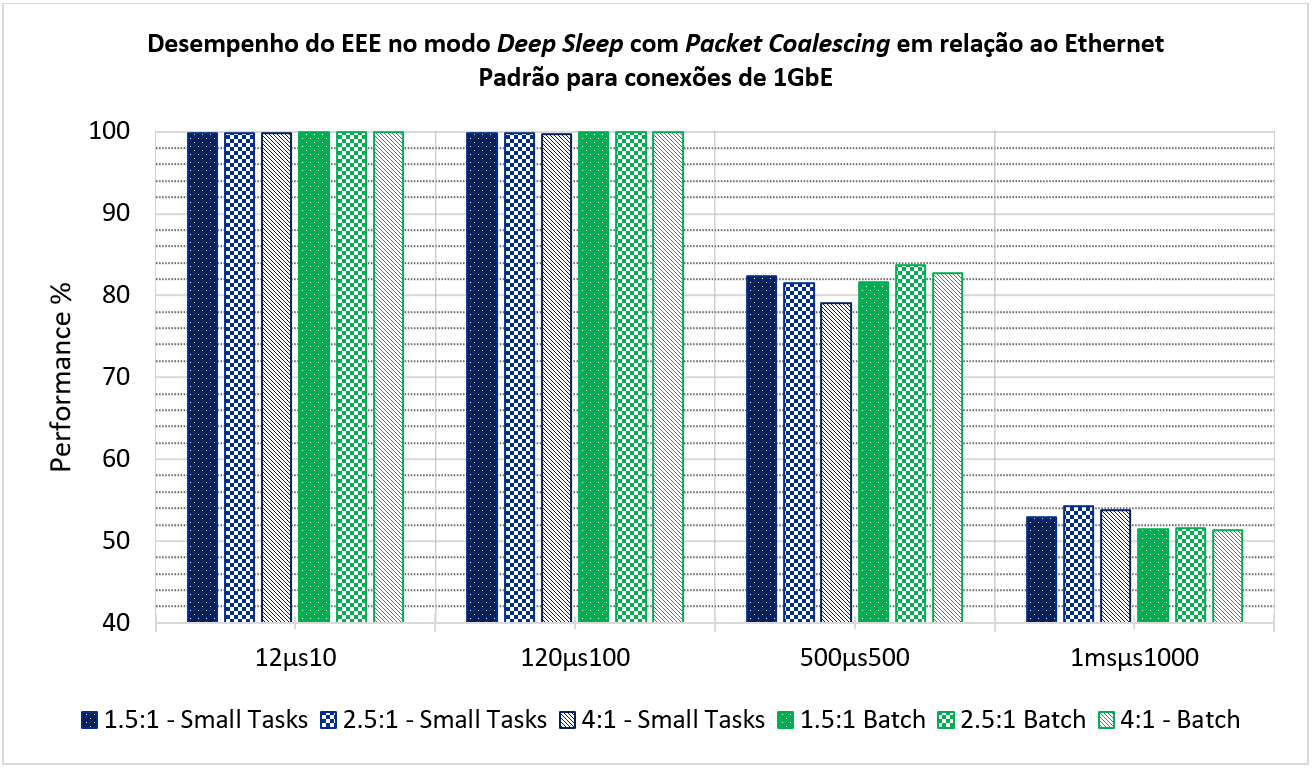
\includegraphics[width=8cm]{5-EEECoDelHadoop/PerfEEEDeepSleepPaco_1GbE.PNG}}\hfill
    \subfloat[\centering Desempenho do EEE no modo \emph{Deep Sleep} com \emph{Packet Coalescing} em relação ao Ethernet Padrão para conexões de 10GbE
    \label{fig:PerfEEEDeepSleepPaCo10GbE}]{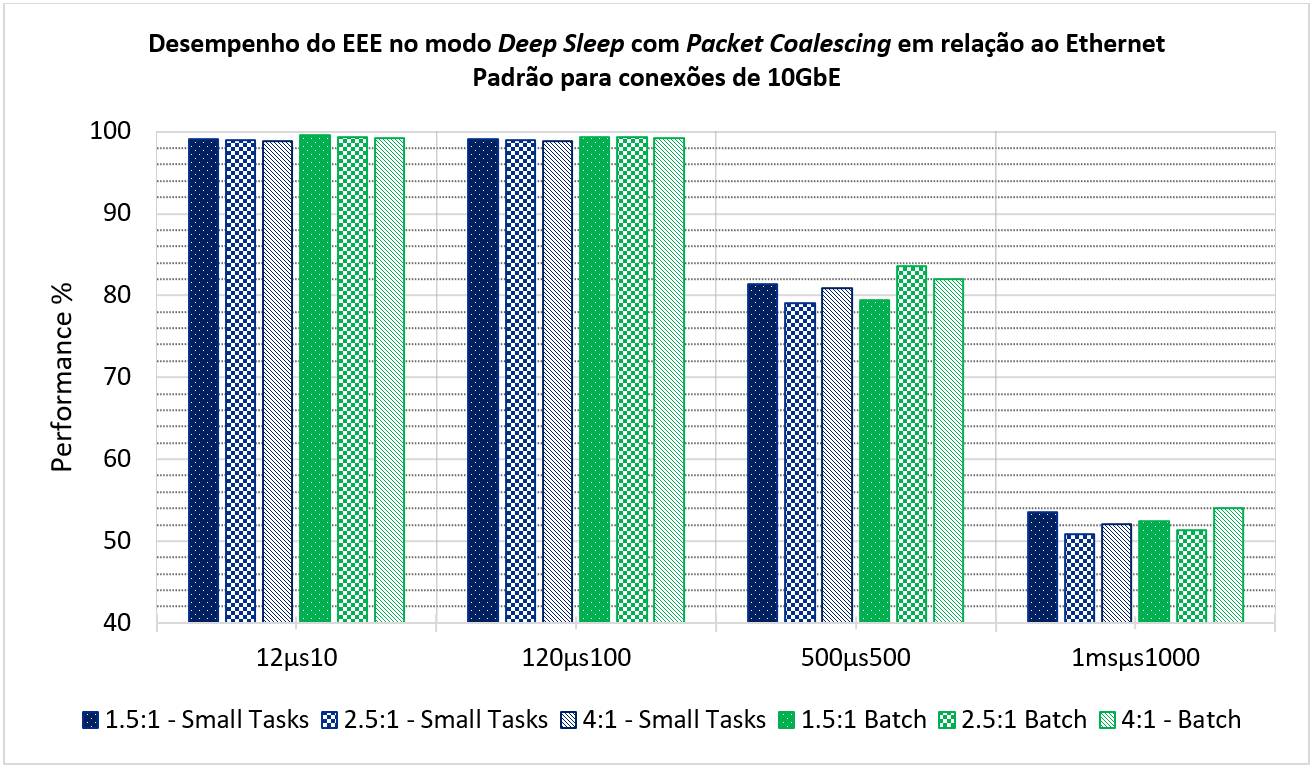
\includegraphics[width=8cm]{5-EEECoDelHadoop/PerfEEEDeepSleepPaco_10GbE.PNG}}
    
    \subfloat[\centering Desempenho do EEE no modo \emph{Deep Sleep} com \emph{Packet Coalescing} em relação ao Ethernet Padrão para conexões de 25GbE \label{fig:PerfEEEDeepSleepPaCo25GbE}]{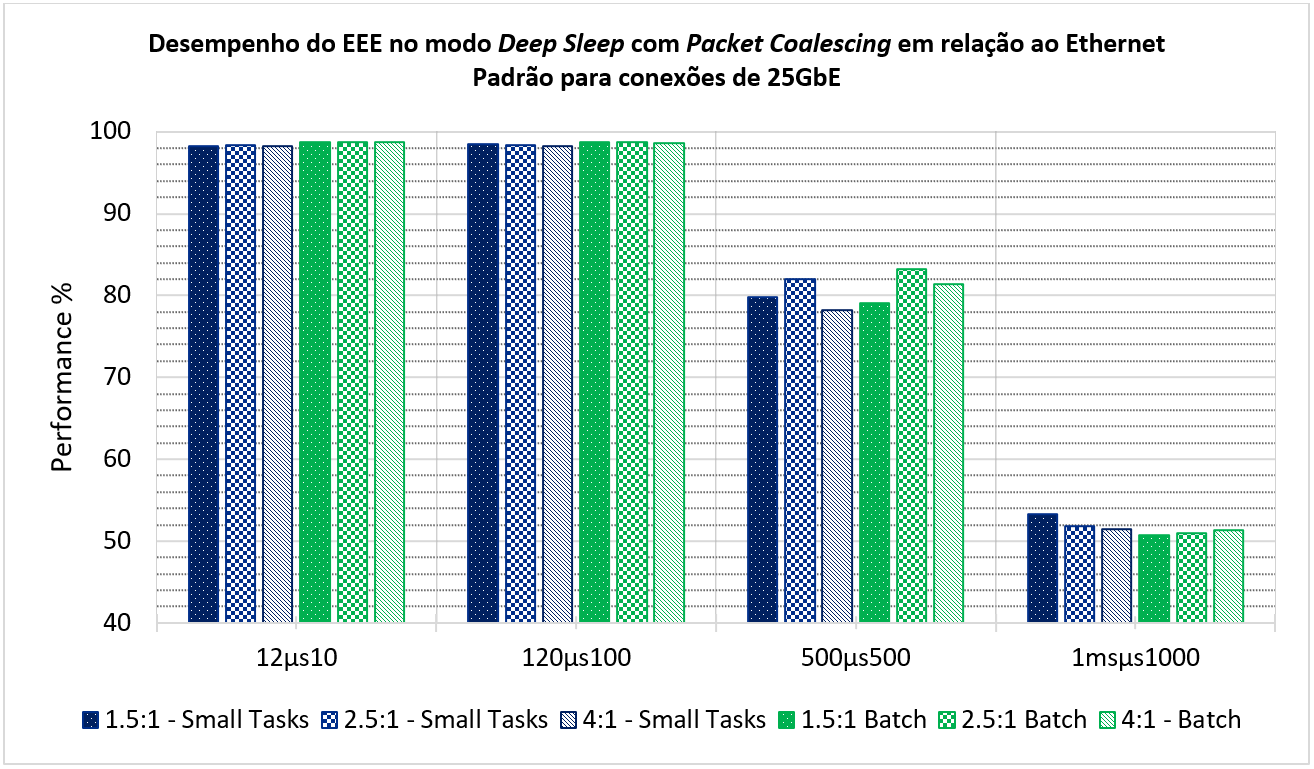
\includegraphics[width=8cm]{5-EEECoDelHadoop/PerfEEEDeepSleepPaco_25GbE.PNG}}\hfill
    \subfloat[\centering Desempenho do EEE no modo \emph{Deep Sleep} com \emph{Packet Coalescing} em relação ao Ethernet Padrão para conexões de 40GbE
    \label{fig:PerfEEEDeepSleepPaCo40GbE}]{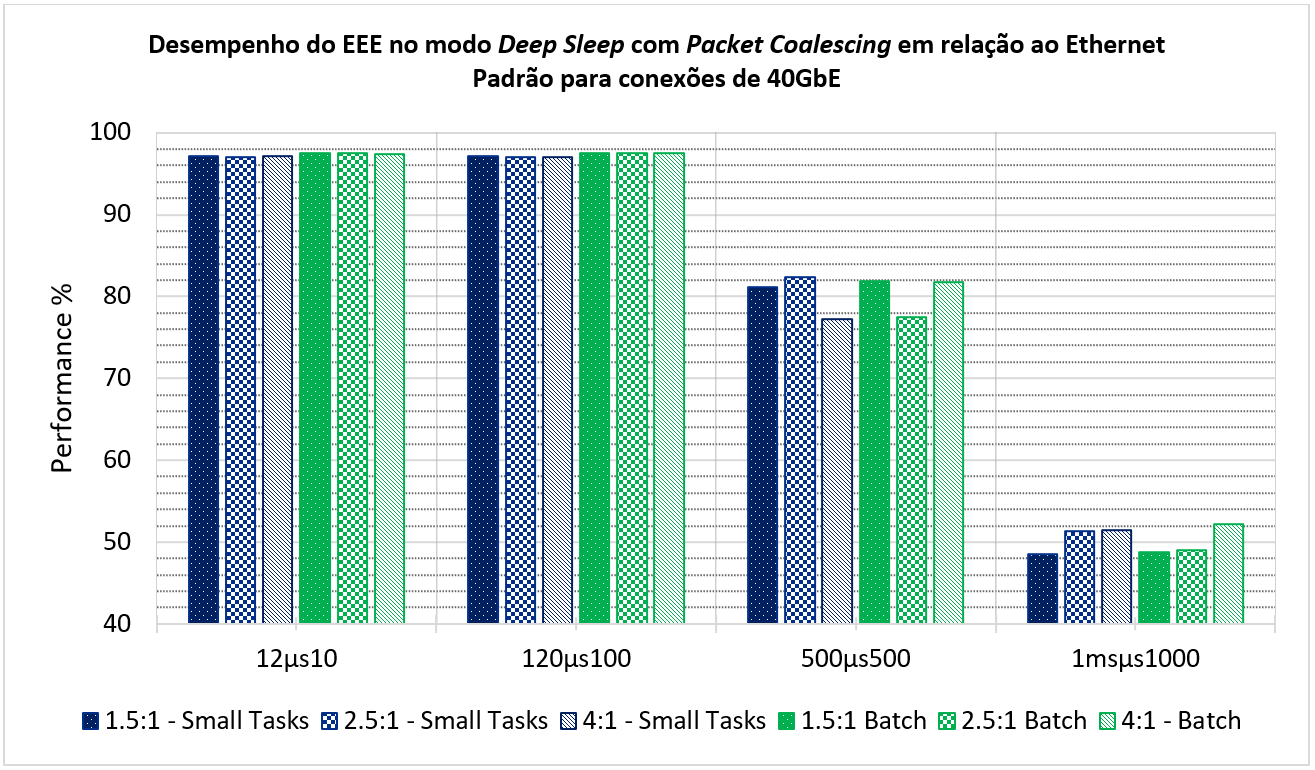
\includegraphics[width=8cm]{5-EEECoDelHadoop/PerfEEEDeepSleepPaco_40GbE.PNG}}    
    
    \subfloat[\centering Desempenho do EEE no modo \emph{Deep Sleep} com \emph{Packet Coalescing} em relação ao Ethernet Padrão para conexões de 100GbE
    \label{fig:PerfEEEDeepSleepPaCo100GbE}]{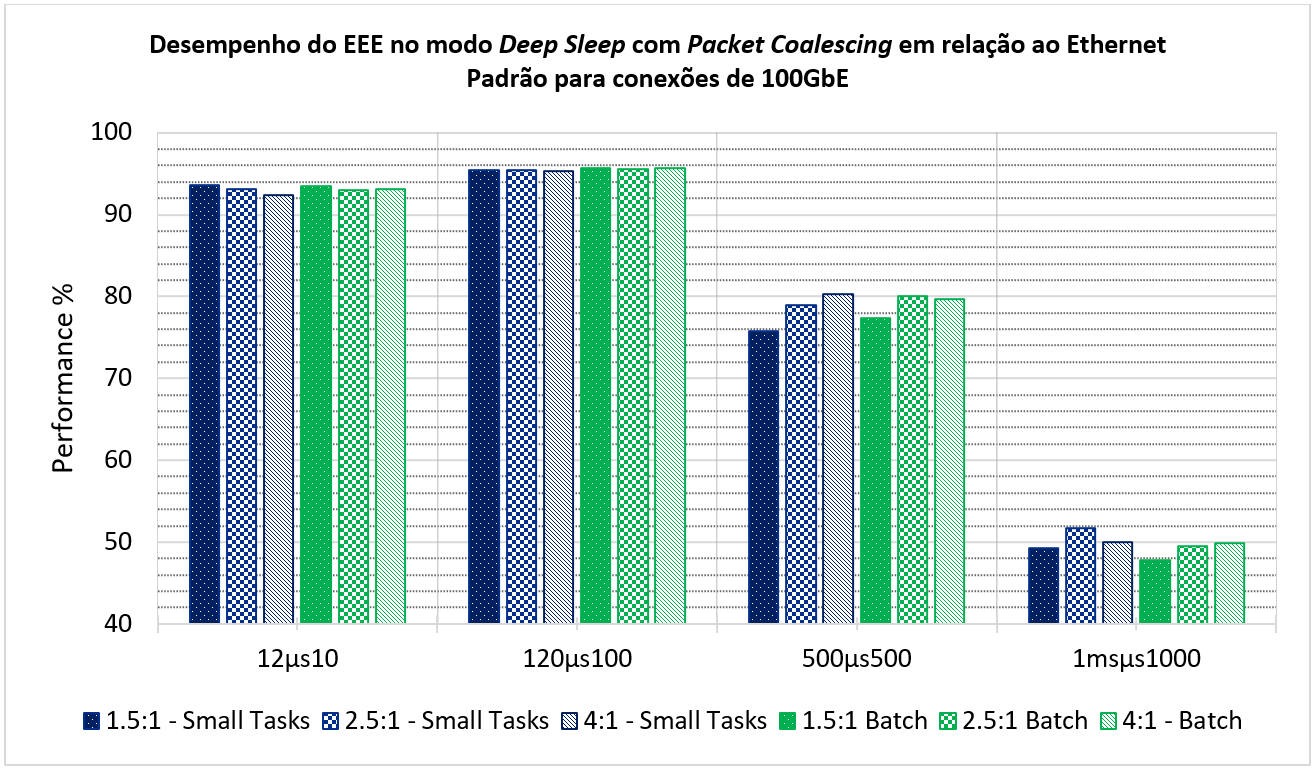
\includegraphics[width=8cm]{5-EEECoDelHadoop/PerfEEEDeepSleepPaco_100GbE.PNG}}\hfill
    \subfloat[\centering Desempenho do EEE no modo \emph{Deep Sleep} com \emph{Packet Coalescing} em relação ao Ethernet Padrão para conexões de 400GbE
    \label{fig:PerfEEEDeepSleepPaCo400GbE}]{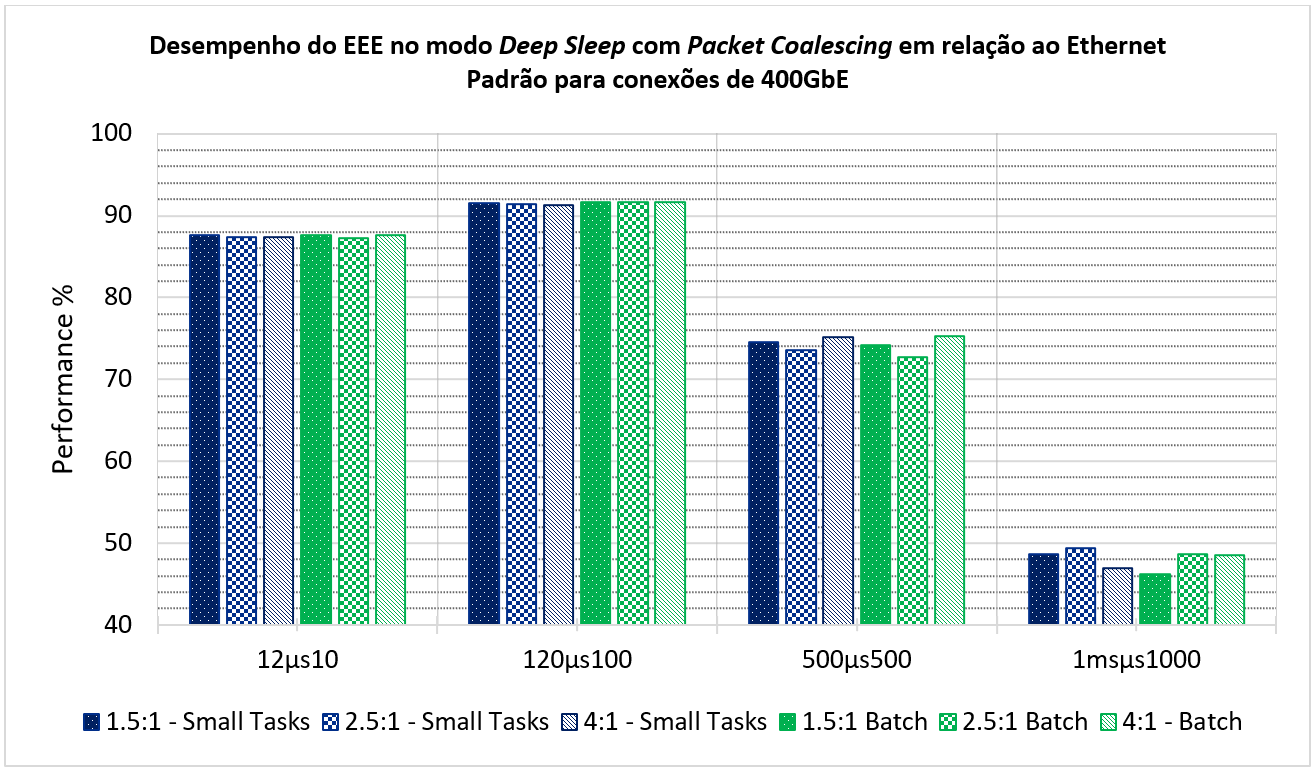
\includegraphics[width=8cm]{5-EEECoDelHadoop/PerfEEEDeepSleepPaco_400GbE.PNG}}       
    
    \caption{\centering Desempenho do EEE no modo \emph{Deep Sleep} com \emph{Packet Coalescing}}
\end{figure}

\begin{figure}[!htb]
    \centering
    \label{fig:PerfEEEFastWakePaCo}
    
    \subfloat[\centering Desempenho do EEE no modo \emph{Fast Wake} com \emph{Packet Coalescing} em relação ao Ethernet Padrão para conexões de 40GbE
    \label{fig:PerfEEEFastWakePaCo40GbE}]{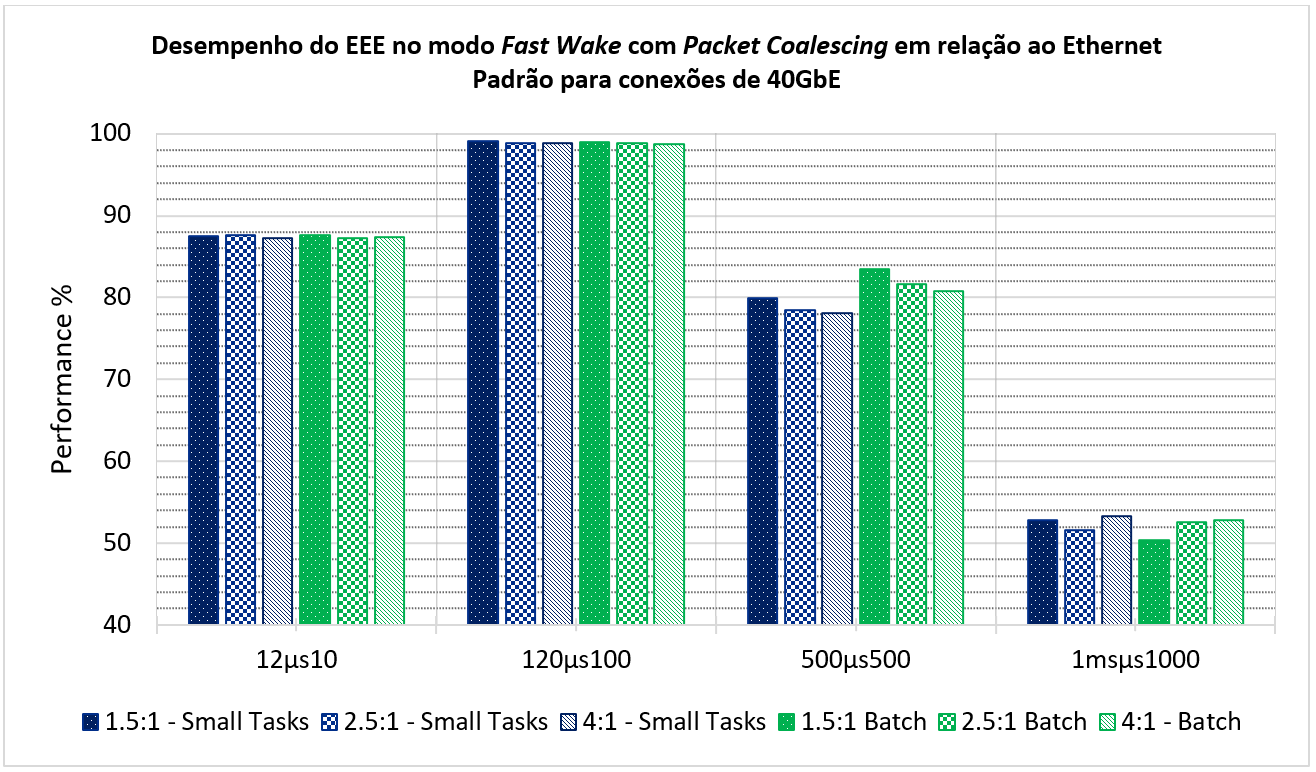
\includegraphics[width=8cm]{5-EEECoDelHadoop/PerfEEEFastWakePaco_40GbE.PNG}}\hfill
    \subfloat[\centering Desempenho do EEE no modo \emph{Fast Wake} com \emph{Packet Coalescing} em relação ao Ethernet Padrão para conexões de 100GbE
    \label{fig:PerfEEEFastWakePaCo100GbE}]{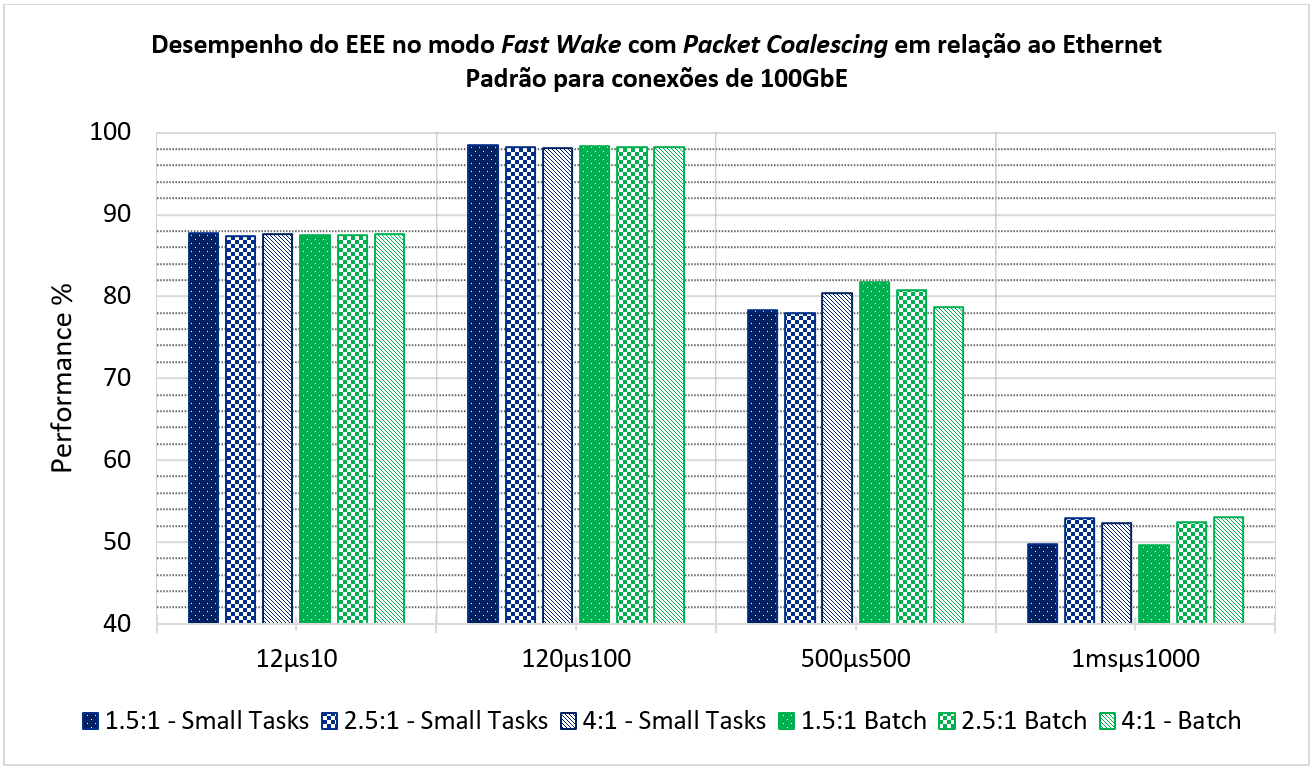
\includegraphics[width=8cm]{5-EEECoDelHadoop/PerfEEEFastWakePaco_100GbE.PNG}}
    
    \caption{\centering Desempenho do EEE no modo \emph{Fast Wake} com \emph{Packet Coalescing}}
\end{figure}

Para as conexões que suportam o EEE no modo \emph{Fast Wake} a configuração 120$\mu$s100 tornou-se a mais crucial, sendo disparadamente a com maior desempenho. No caso das conexões de 40GbE, o desempenho manteve-se estável de 98.8\% para 98.89\%, enquanto em links de 400GbE foi de 98.2\% para 98.28\%. Ao utilizarmos configurações como 12$\mu$s10, o desempenho degradou-se para 87.466\% e 87.52\% respectivamente, só não sendo pior que o desempenho de 1ms1000, que atingiu valores de 52.228\% e 51.649\%. Como esperado, a performance dos \emph{Batch Jobs} foram vagamente melhores.

Durante nossas simulações quatro diferentes configurações para o \emph{Packet Coalescing} foram testadas, 12$\mu$s10, 120$\mu$s100, 500$\mu$s500 e 1ms1000. A primeira demonstrou-se ser de certa forma eficaz em manter a performance em conexões até 40GbE, entretanto ao irmos para conexões maiores como 100GbE e 400GbE tornou-se necessário a utilização da segunda configuração para manter o desempenho. Em contrapartida, a terceira e quarta configurações demonstraram uma degradação grande da performance, sendo assim descartadas. Ao avaliarmos o contexto de \textbf{economia de energia x performance}, optamos pela escolha da configuração 120$\mu$s100 para ser a padrão nos próximos testes que envolvem \emph{Packet Coalescing} combinado com CoDel, RED e ECN.

\section{Energy Efficient Ethernet com Packet Coalescing, Controlled Delay e Explicit Congestion Notification}

Na seção anterior demonstramos através dos resultados como a utilização de \emph{Packet Coalescing} configurado corretamente e combinado com \emph{Energy Efficient Ethernet} pode reduzir ainda mais o consumo de energia sem degradação agressiva da performance do \emph{cluster}. Nesta seção apresentamos os resultados de nossas tentativas de combinar \emph{Energy Efficient Ethernet}, \emph{Packet Coalescing}, \emph{Controlled Delay} e \emph{Explicit Congestion Notification} para melhorar a performance. A metodologia detalhada das configurações pode ser observada no Capítulo 3.


\subsection{Economia de Energia}

\begin{figure}[!htb]
    \centering
    \label{fig:EEEDeepSleepPaCoCoDelECN}
    
    \subfloat[\centering Consumo de energia do EEE no modo \emph{Deep Sleep} com \emph{Packet Coalescing}, CoDeL e ECN em conexões de 1GbE \label{fig:EEEDeepSleepPaCoCoDelECN1GbE}]{\includegraphics[width=8cm]{5-EEECoDelHadoop/EEEDeepSleepPaCoCoDelECN_1GbE.PNG}}\hfill
    \subfloat[\centering Consumo de energia do EEE no modo \emph{Deep Sleep} com \emph{Packet Coalescing}, CoDeL e ECN em conexões de 10GbE
    \label{fig:EEEDeepSleepPaCoCoDelECN10GbE}]{\includegraphics[width=8cm]{5-EEECoDelHadoop/EEEDeepSleepPaCoCoDelECN_10GbE.PNG}}
    
    \subfloat[\centering Consumo de energia do EEE no modo \emph{Deep Sleep} com \emph{Packet Coalescing}, CoDeL e ECN em conexões de 25GbE \label{fig:EEEDeepSleepPaCoCoDelECN25GbE}]{\includegraphics[width=8cm]{5-EEECoDelHadoop/EEEDeepSleepPaCoCoDelECN_25GbE.PNG}}\hfill
    \subfloat[\centering Consumo de energia do EEE no modo \emph{Deep Sleep} com \emph{Packet Coalescing}, CoDeL e ECN em conexões de 40GbE
    \label{fig:EEEDeepSleepPaCoCoDelECN40GbE}]{\includegraphics[width=8cm]{5-EEECoDelHadoop/EEEDeepSleepPaCoCoDelECN_40GbE.PNG}}    
    
    \subfloat[\centering Consumo de energia do EEE no modo \emph{Deep Sleep} com \emph{Packet Coalescing}, CoDeL e ECN em conexões de 100GbE
    \label{fig:EEEDeepSleepPaCoCoDelECN100GbE}]{\includegraphics[width=8cm]{5-EEECoDelHadoop/EEEDeepSleepPaCoCoDelECN_100GbE.PNG}}\hfill
    \subfloat[\centering Consumo de energia do EEE no modo \emph{Deep Sleep} com \emph{Packet Coalescing}, CoDeL e ECN em conexões de 400GbE
    \label{fig:EEEDeepSleepPaCoCoDelECN400GbE}]{\includegraphics[width=8cm]{5-EEECoDelHadoop/EEEDeepSleepPaCoCoDelECN_400GbE.PNG}}       
    
    \caption{\centering Consumo de energia do EEE no modo \emph{Deep Sleep} com \emph{Packet Coalescing}, CoDeL e ECN}
\end{figure}


\begin{figure}[!htb]
    \centering
    \label{fig:EEEFastWakePaCoCoDelECN}
    
    \subfloat[\centering Consumo de energia do EEE no modo \emph{Fast Wake} com \emph{Packet Coalescing}, CoDeL e ECN em conexões de 40GbE
    \label{fig:EEEFastWakePaCoCoDelECN40GbE}]{\includegraphics[width=8cm]{5-EEECoDelHadoop/EEEFastWakePaCoCoDelECN_40GbE.PNG}}\hfill
    \subfloat[\centering Consumo de energia do EEE no modo \emph{Fast Wake} com \emph{Packet Coalescing}, CoDeL e ECN em conexões de 100GbE
    \label{fig:EEEFastWakePaCoCoDelECN100GbE}]{\includegraphics[width=8cm]{5-EEECoDelHadoop/EEEFastWakePaCoCoDelECN_100GbE.PNG}}
    
    \caption{\centering Consumo de energia do EEE no modo \emph{Fast Wake} com \emph{Packet Coalescing}, CoDeL e ECN}
\end{figure}

As figuras 5.5 e 5.6 ilustram os resultados das simulações. De forma geral a agregação do \emph{Controlled Delay} não alterou o consumo de energia significativamente. Em conexões de 1GbE demonstrou-se mais uma vez ser desnecessário a implementação de recursos como \emph{Packet Coalescing}, tendo uma redução de 16.11\% (0.0805 w/h) para 15.95\% (0.0798 w/h) em relação ao Ethernet padrão na melhor das configurações, 400$\mu$s1ms.

Nas conexões de 10GbE o melhor valor foi obtido na configuração 800$\mu$s1.5ms, com um consumo reduzido de 18.32\% (0.4909 w/h) para 11.69\% (0.3134 w/h) em relação ao Ethernet padrão. Para os links de 25GbE, o melhor consumo foi anotado ao usarmos 300$\mu$s0.75$\mu$s, reduzindo de 19.82\% (1.0725 w/h) para 13.22\% (0.715 w/h).

Em links de 40GbE todas as configurações se mantiveram com um mesmo padrão de consumo de energia, cerca de 13.1\%, o que representa 0.98 w/h. Para os links de 100GbE o melhor consumo foi obtido ao utilizar a configuração 400$\mu$s1ms, reduzindo o consumo de 24.31\% (2.6469 w/h) para 15.58\% (1.6853 w/h).

Por fim, para conexões de 400GbE a melhor configuração foi 400$\mu$s1ms, reduzindo o consumo de energia de 48.11\% (10.6853 w/h) para 25.54\% (5.6724 w/h). Em contrapartida, a pior configuração para esta configuração foi de 800$\mu$s1.5ms, atingindo um consumo de energia de 25.68\% (5.7036 w/h).

Ao habilitarmos a tecnologia \emph{Fast Wake} no EEE para conexões de 40GbE e 100GbE com \emph{Packet Coalescing}, CoDel e ECN também foi possível notar leves diferenças no consumo de energia, como a redução de 61.87\% (4.6340 w/h) e 63.51\% (9.9160) para 39.8\% (2.9814 w/h) e 39.81\% (4.3357 w/h) em configurações de 800$\mu$s1.5ms.

Uma paridade entre os consumos de energia do EEE com \emph{Packet Coalescing} e EEE com \emph{Packet Coalescing}, CoDel e ECN já era esperada, uma vez que o foco principal deste algoritmo é melhorar o desempenho do \emph{cluster}, e não a economia de energia em si.


\subsection{Desempenho}

Esta subseção contém os resultados da performance das simulações - fator principal para aplicar o \emph{Controlled Delay} juntamente ao \emph{Packet Coalescing} e \emph{Explicit Congestion Notification}. Em conexões de 1GbE a melhor performance de 99.88\% foi obtida ao utilizarmos a configuração 800$\mu$s1.5ms. Comparado ao Ethernet padrão, a performance deste link era de 99.78\% com apenas o EEE. Já a pior performance foi encontrada ao usarmos a configuração 400$\mu$s1ms, chegando à 99.86\%.

Para os links de 10GbE obtivemos uma média de performance melhor com a configuração 800$\mu$s1.5ms, aumentando a performance de 99.054\% para 99.1535\%. Por outro lado, o posto de pior configuração ficou com as demais configurações 500$\mu$s20ms, 300$\mu$s0.75$\mu$s e 400$\mu$s1m, que atingiram uma média de performance de 99.14\%.

Conforme avançamos nos testes para conexões com uma maior banda ficou claro como uma boa configuração do CoDel com ECN impactava no desempenho do \emph{cluster}. Para os links de 25GbE, o melhor desempenho de 98.673\% foi alcançando ao usarmos a configuração 800$\mu$s1.5ms, e a pior de 98.549\% ao usar como parâmetro 400$\mu$s1ms.

Nas simulações à partir de 40GbE já ficavam claras a melhor e pior configuração dentre as opções adotadas dentro da bibliografia disponível, 800$\mu$s1.5ms e 400$\mu$s1ms. Na conexão de 40GbE, o melhor parâmetro 800$\mu$s1.5ms foi responsável por elevar a performance de 97.147\% para 97.521\%, enquanto o pior parâmetro 400$\mu$s1ms atingiu 97.284\%.

Ao considerarmos conexões maiores como 100GbE e 400GbE a diferença de performance entre os parâmetros se tornou ainda maior. No caso dos links de 100GbE a melhor configuração 800$\mu$s1.5ms obteve uma performance de 95.97\%, contra 95.57\% da pior 400$\mu$s1ms. A performance com EEE padrão para este link é de 95.44\%. Em conexões de 400GbE a performance foi ligeiramente aumentada de 91.413\% para 92.32\% com o melhor parâmetro 800$\mu$s1.5ms, e manteve-se em 91.58\% com 400$\mu$s1ms.

Com a tecnologia \emph{Fast Wake} do EEE também foram realizadas simulações. Entretanto, notamos que ao adicionar o \emph{Packet Coalescing} juntamente ao CoDel e ECN houve uma degradação da performance.  Para conexões de 40GbE, mesmo com a nossa melhor configuração 800$\mu$s1.5ms a performance caiu para 95.962\%, e ainda mais, para 95.577\% quando utilizamos o pior parâmetro dentro das opções 400$\mu$s1ms.

\begin{figure}[!htb]
    \centering
    \label{fig:PerfEEEDeepSleepPaCoCoDelECN}
    
    \subfloat[\centering Desempenho do EEE no modo \emph{Deep Sleep} com \emph{Packet Coalescing}, CoDel e ECN em relação ao Ethernet Padrão para conexões de 1GbE
    \label{fig:PerfEEEDeepSleepPaCoCoDelECN1GbE}]{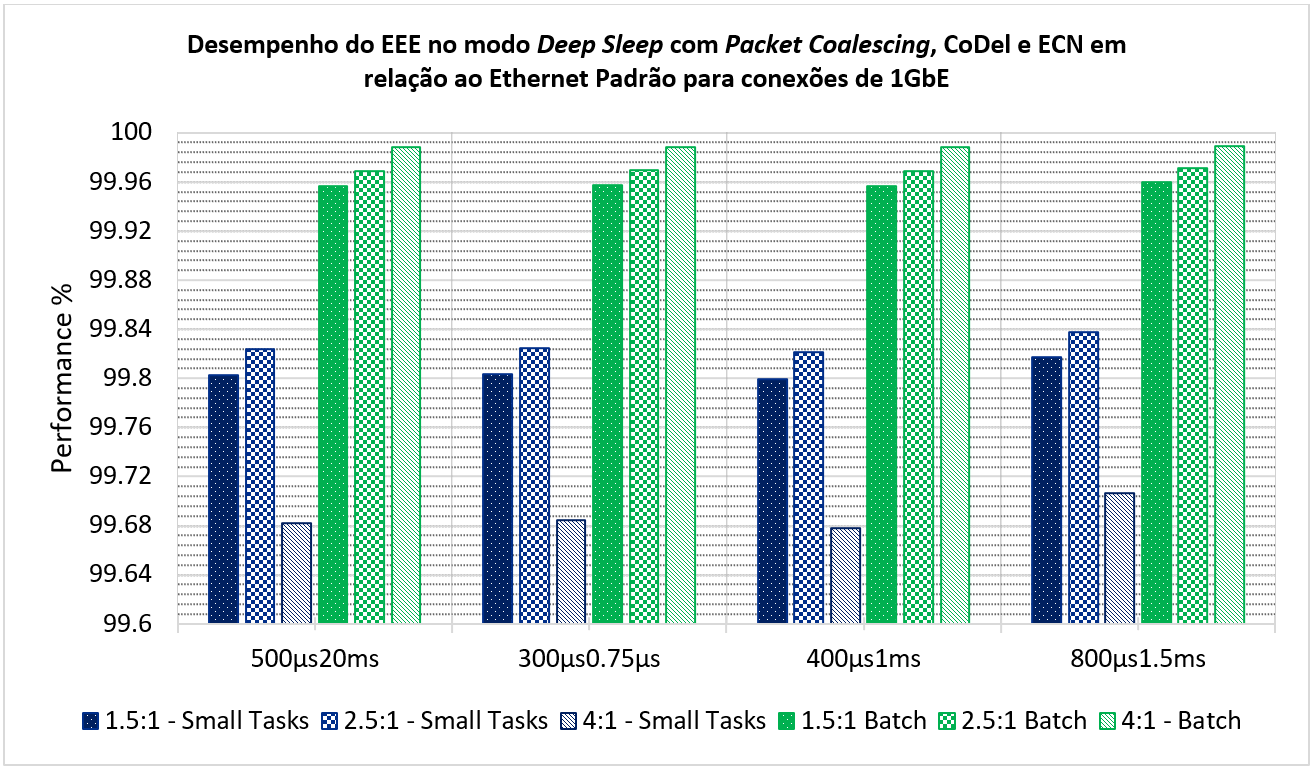
\includegraphics[width=8cm]{5-EEECoDelHadoop/PerfEEEDeepSleepPacoCoDelECN_1GbE.PNG}}\hfill
    \subfloat[\centering Desempenho do EEE no modo \emph{Deep Sleep} com \emph{Packet Coalescing}, CoDel e ECN em relação ao Ethernet Padrão para conexões de 10GbE
    \label{fig:PerfEEEDeepSleepPaCoCoDelECN10GbE}]{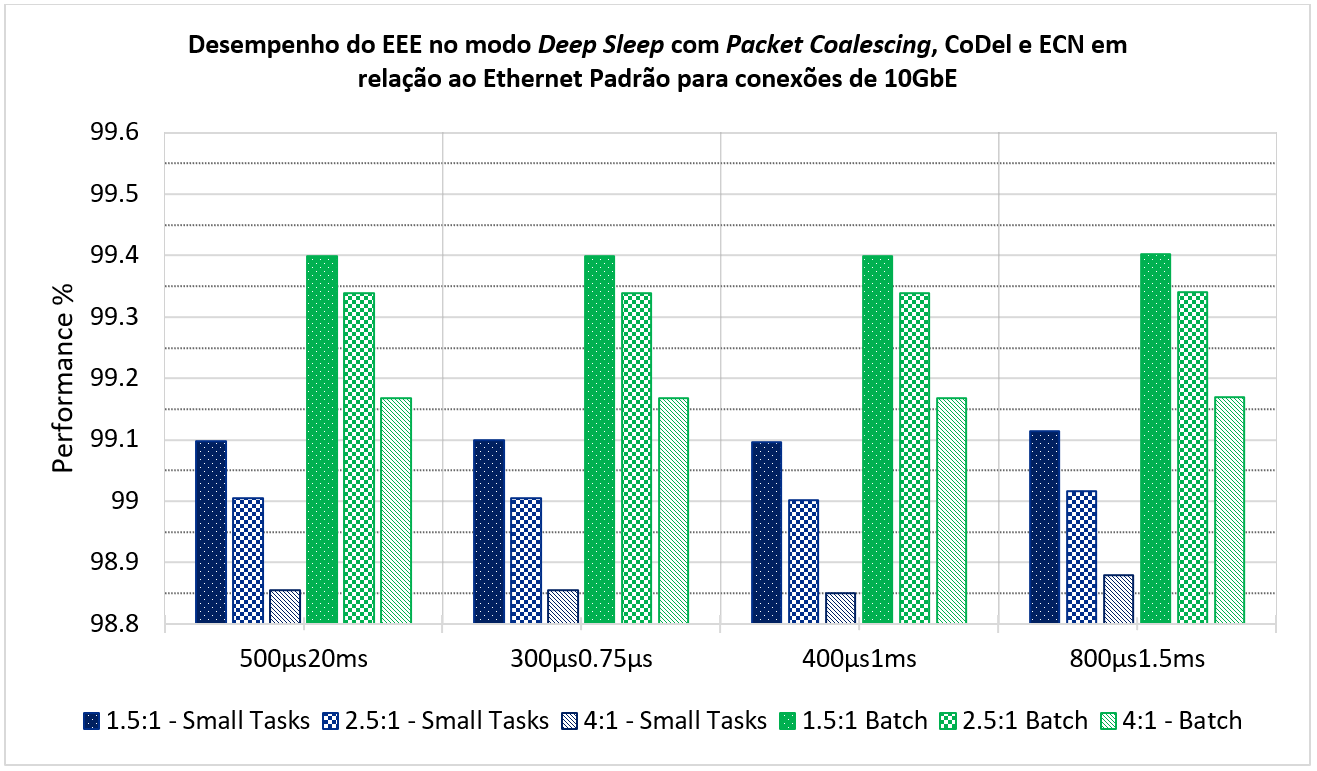
\includegraphics[width=8cm]{5-EEECoDelHadoop/PerfEEEDeepSleepPacoCoDelECN_10GbE.PNG}}
    
    \subfloat[\centering Desempenho do EEE no modo \emph{Deep Sleep} com \emph{Packet Coalescing}, CoDel e ECN em relação ao Ethernet Padrão para conexões de 25GbE \label{fig:PerfEEEDeepSleepPaCoCoDelECN25GbE}]{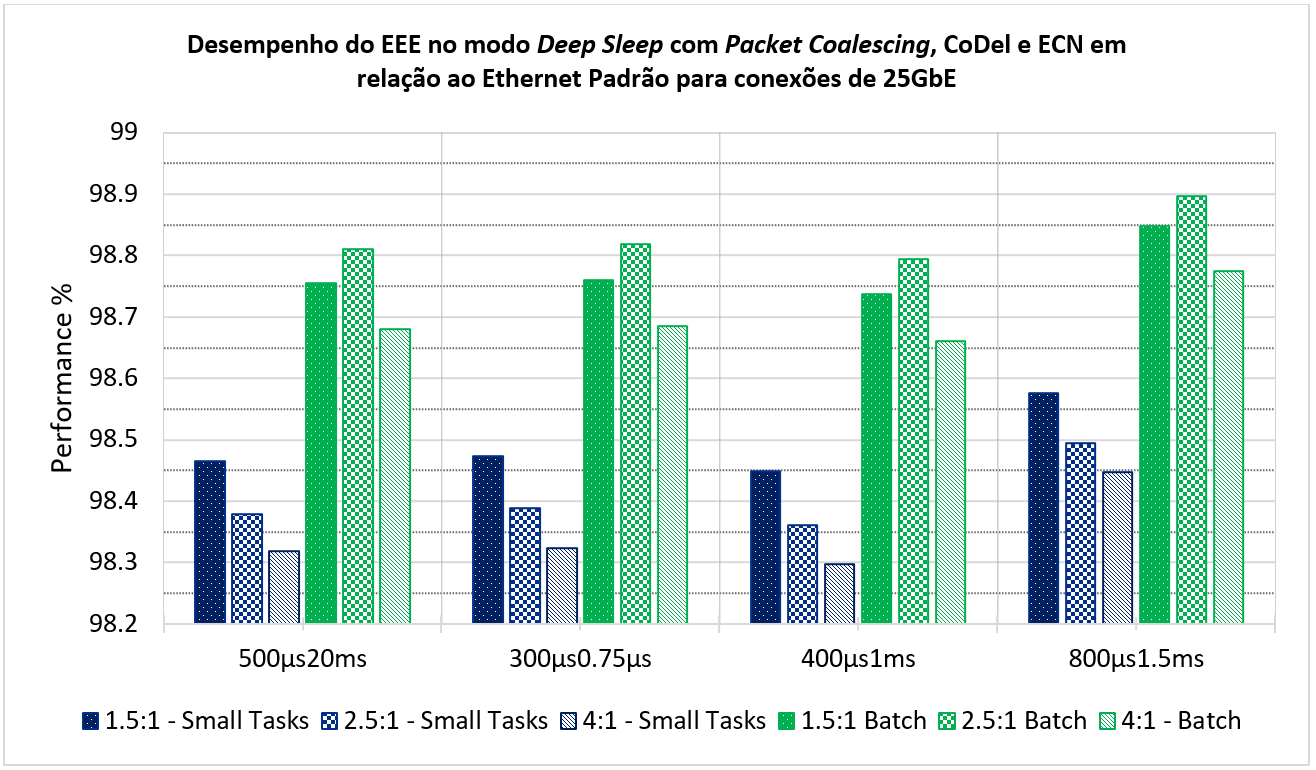
\includegraphics[width=8cm]{5-EEECoDelHadoop/PerfEEEDeepSleepPacoCoDelECN_25GbE.PNG}}\hfill
    \subfloat[\centering Desempenho do EEE no modo \emph{Deep Sleep} com \emph{Packet Coalescing}, CoDel e ECN em relação ao Ethernet Padrão para conexões de 40GbE
    \label{fig:PerfEEEDeepSleepPaCoCoDelECN40GbE}]{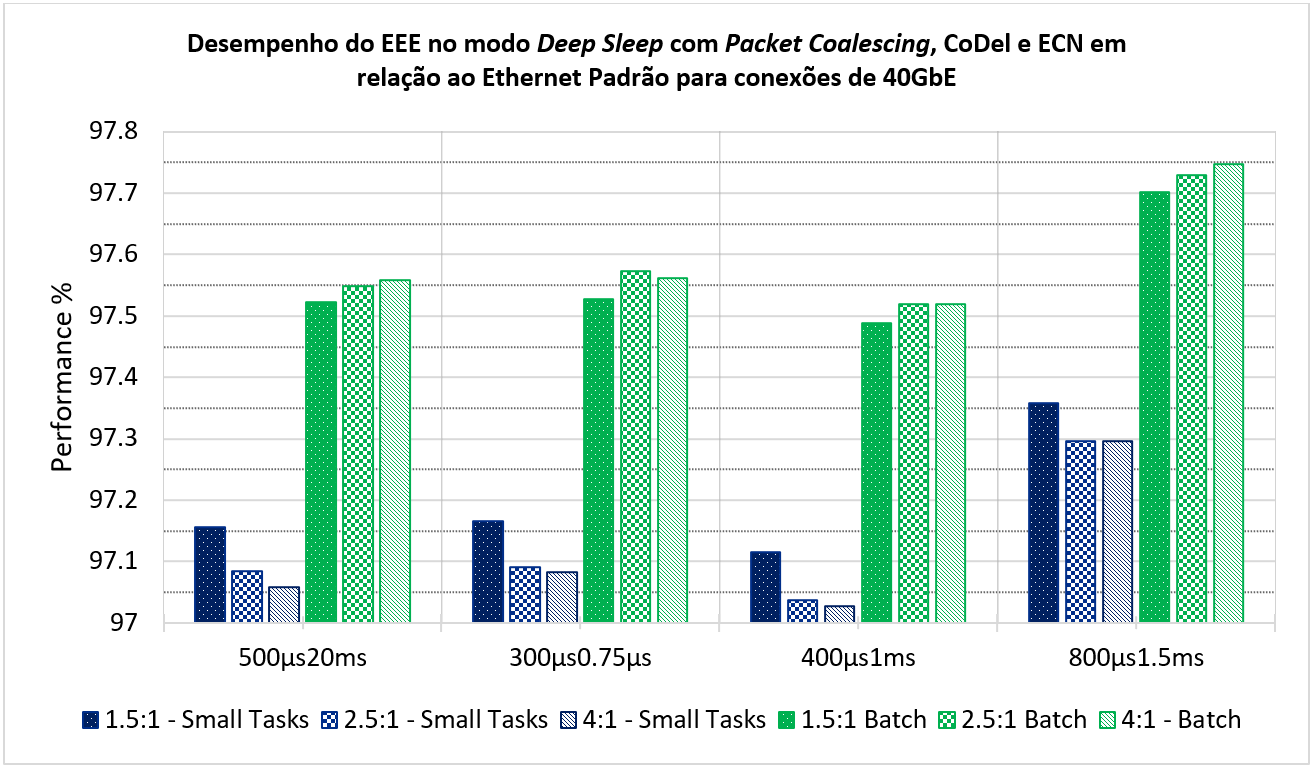
\includegraphics[width=8cm]{5-EEECoDelHadoop/PerfEEEDeepSleepPacoCoDelECN_40GbE.PNG}}    
    
    \subfloat[\centering Desempenho do EEE no modo \emph{Deep Sleep} com \emph{Packet Coalescing}, CoDel e ECN em relação ao Ethernet Padrão para conexões de 100GbE
    \label{fig:PerfEEEDeepSleepPaCoCoDelECN100GbE}]{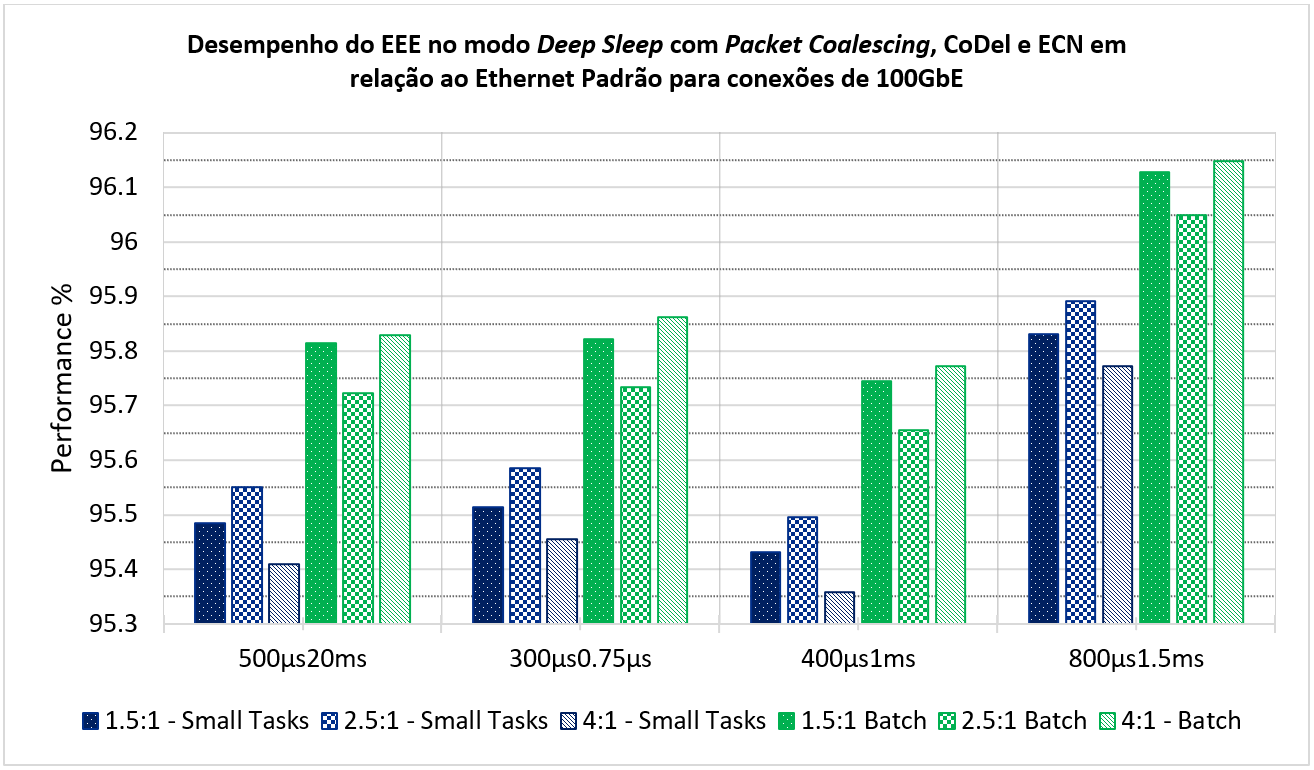
\includegraphics[width=8cm]{5-EEECoDelHadoop/PerfEEEDeepSleepPacoCoDelECN_100GbE.PNG}}\hfill
    \subfloat[\centering Desempenho do EEE no modo \emph{Deep Sleep} com \emph{Packet Coalescing}, CoDel e ECN em relação ao Ethernet Padrão para conexões de 400GbE
    \label{fig:PerfEEEDeepSleepPaCoCoDelECN400GbE}]{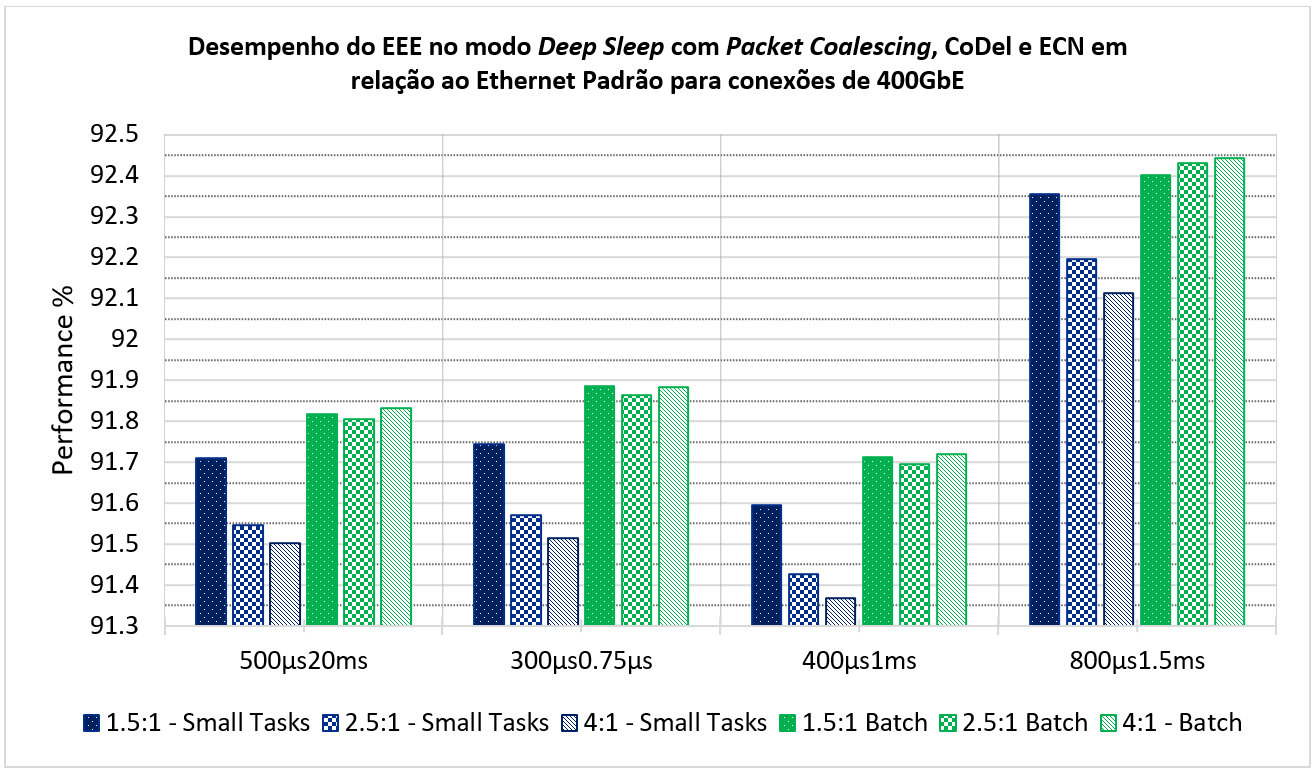
\includegraphics[width=8cm]{5-EEECoDelHadoop/PerfEEEDeepSleepPacoCoDelECN_400GbE.PNG}}       
    
    \caption{\centering Desempenho do EEE no modo \emph{Deep Sleep} com \emph{Packet Coalescing}, CoDel e ECN}
\end{figure}

Dentre os resultados obtidos, consideramos interessante a aplicação do \emph{Packet Coalescing} com \emph{Controlled Delay} e \emph{Explicit Congestion Notification} em conexões EEE no modo \emph{Deep Sleep} superiores à 40GbE, principalmente quando os parâmetros adequados para tais conexões são encontrados como foi o caso de 800$\mu$s1.5ms.

Ao utilizarmos o modo \emph{Fast Wake} do EEE com \emph{Packet Coalescing}, \emph{Controlled Delay} e \emph{Explicit Congestion Notification} houve uma degradação considerável da performance em relação ao EEE no modo \emph{Fast Wake} com apenas \emph{Packet Coalescing}. Isso se deve ao fato do \emph{Controlled Delay} adicionar uma latência extra superior a própria latência do EEE no modo \emph{Fast Wake} agravando a congestão do tráfego \cite{silva2018eon}; \cite{silva2016controlling}; \cite{e2019tcp}.

\begin{figure}[!htb]
    \centering
    \label{fig:PerfEEEFastWakePaCoCodelECN}
    
    \subfloat[\centering Desempenho do EEE no modo \emph{Fast Wake} com \emph{Packet Coalescing}, CoDel e ECN em relação ao Ethernet Padrão para conexões de 40GbE
    \label{fig:PerfEEEFastWakePaCoCoDelECN40GbE}]{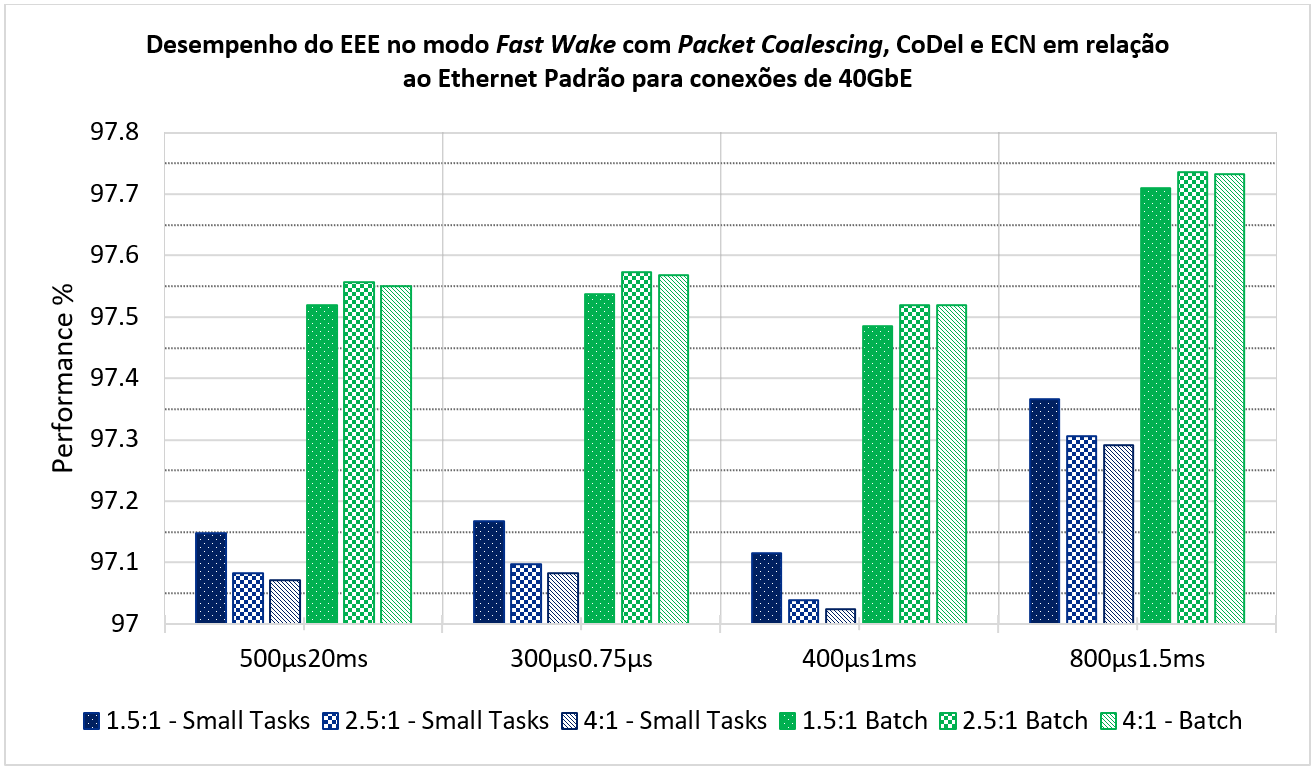
\includegraphics[width=8cm]{5-EEECoDelHadoop/PerfEEEFastWakePacoCoDelECN_40GbE.PNG}}\hfill
    \subfloat[\centering Desempenho do EEE no modo \emph{Fast Wake} com \emph{Packet Coalescing}, CoDel e ECN em relação ao Ethernet Padrão para conexões de 100GbE
    \label{fig:PerfEEEFastWakePaCoCoDelECN100GbE}]{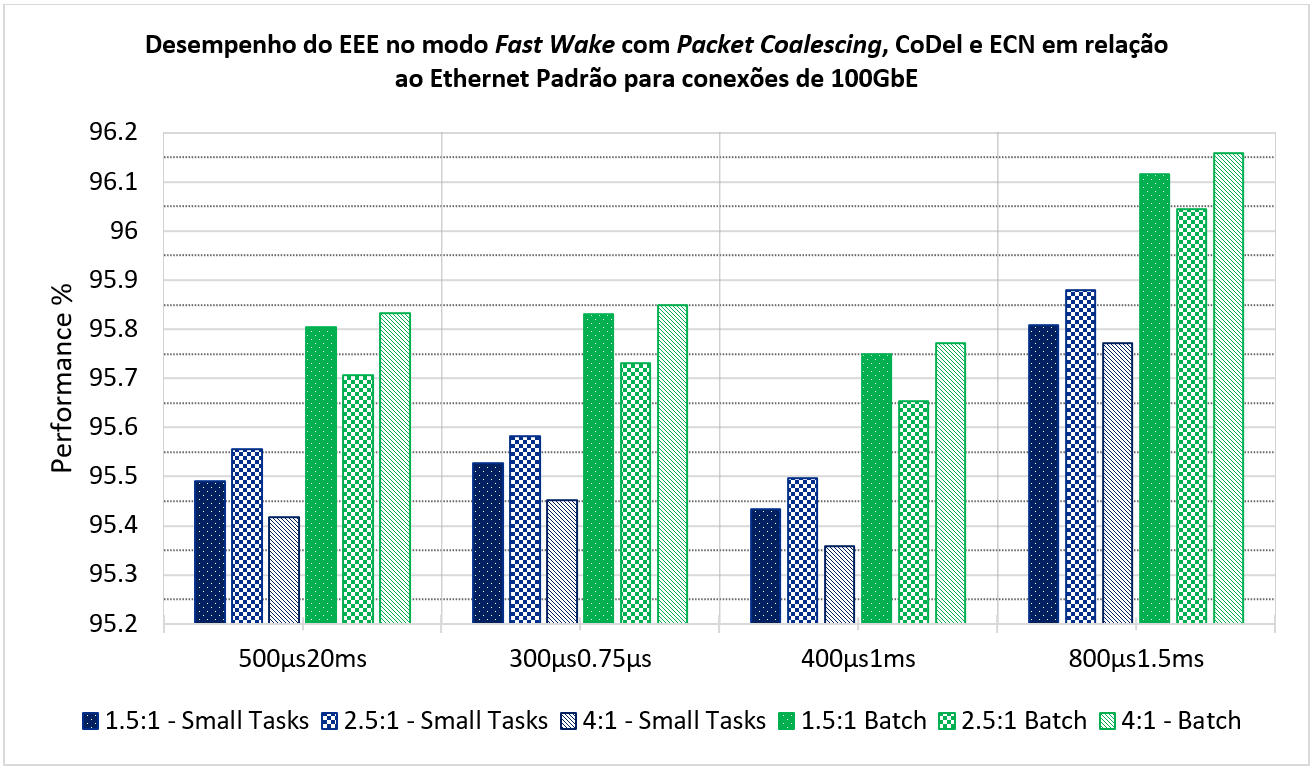
\includegraphics[width=8cm]{5-EEECoDelHadoop/PerfEEEFastWakePacoCoDelECN_100GbE.PNG}}
    
    \caption{\centering Desempenho do EEE no modo \emph{Fast Wake} com \emph{Packet Coalescing}, CoDel e ECN}
\end{figure}



\section{Energy Efficient Ethernet com Packet Coalescing, Random Early Detection e Explicit Congestion Notification}

Esta seção apresenta os resultados das simulações em que combinamos \emph{Packet Coalescing} com \emph{Random Early Detection} e \emph{Congestion Notification}, e investigamos como projetar e configurar conexões EEE para fornecer o máximo de economia de energia sem degradar o desempenho do \emph{cluster}. Como mencionado anteriormente durante nossas simulações quatro diferentes configurações para o \emph{Packet Coalescing} foram testadas, 12$\mu$s10, 120$\mu$s100, 500$\mu$s500 e 1ms1000, e optamos pela escolha da configuração 120$\mu$s100 para ser a padrão nos testes que envolvem \emph{Packet Coalescing} combinado, RED e ECN por ser a que manteve a performance e forneceu uma melhor economia de energia para as conexões.

A metodologia detalhada das configurações pode ser observada no Capítulo 3. Consideramos \emph{Random Early Detection} como o \emph{Active Queue Management} selecionado para marcar pacotes com recurso \emph{Explicit Congestion Notification} configurado em remetentes TCP, e definimos os valores baseados em trabalhos anteriores, como 70 {$\mathit{Min}_\mathit{th}$} e 70 {$\mathit{Max}_\mathit{th}$}  em \cite{alizadeh2010data}; 125 {$\mathit{Min}_\mathit{th}$} e 375 {$\mathit{Max}_\mathit{th}$}, 25 {$\mathit{Min}_\mathit{th}$} e 75 {$\mathit{Max}_\mathit{th}$}, 50 {$\mathit{Min}_\mathit{th}$} e 150 {$\mathit{Max}_\mathit{th}$} em \cite{silva2018eon}.

\subsection{Economia de Energia}

Os resultados das simulações de economia de energia com EEE nos modos \emph{Deep Sleep} e \emph{Fast Wake} combinados com RED e ECN podem ser observados nas figuras 5.9 e 5.10. Uma paridade envolvendo os resultados somente com \emph{Packet Coalescing} e \emph{Packet Coalescing} com RED era esperada, isso porque o RED é um algoritmo focado em ganho de desempenho.

Como pode-se observar na figura 5.9, em links de 1GbE acontece uma pequena redução do consumo de energia em relação ao EEE padrão, de 16.11\% (0.0805 w/h) para 15.76\% (0.0788 w/h) ao usarmos a configuração do RED em 70{$\mathit{Min}_\mathit{th}$}70{$\mathit{Max}_\mathit{th}$}.

Para as conexões de 10GbE encontramos uma redução no consumo de energia de 18.32\% (0.4909 w/h) para 11.53\% (0.3091 w/h) ao aplicar a configuração 25{$\mathit{Min}_\mathit{th}$}75{$\mathit{Max}_\mathit{th}$}. A pior configuração para esta conexão 125{$\mathit{Min}_\mathit{th}$}375{$\mathit{Max}_\mathit{th}$} forneceu um consumo de 11.60\% (0.3110 w/h).

\begin{figure}[!htb]
    \centering
    \label{fig:EEEDeepSleepPaCoREDECN}
    
    \subfloat[\centering Consumo de energia do EEE no modo \emph{Deep Sleep} com \emph{Packet Coalescing}, RED e ECN em conexões de 1GbE \label{fig:EEEDeepSleepPaCoREDECN1GbE}]{\includegraphics[width=8cm]{5-EEECoDelHadoop/EEEDeepSleepPaCoREDECN_1GbE.PNG}}\hfill
    \subfloat[\centering Consumo de energia do EEE no modo \emph{Deep Sleep} com \emph{Packet Coalescing}, RED e ECN em conexões de 10GbE
    \label{fig:EEEDeepSleepPaCoREDECN10GbE}]{\includegraphics[width=8cm]{5-EEECoDelHadoop/EEEDeepSleepPaCoREDECN_10GbE.PNG}}
    
    \subfloat[\centering Consumo de energia do EEE no modo \emph{Deep Sleep} com \emph{Packet Coalescing}, RED e ECN em conexões de 25GbE \label{fig:EEEDeepSleepPaCoREDECN25GbE}]{\includegraphics[width=8cm]{5-EEECoDelHadoop/EEEDeepSleepPaCoREDECN_25GbE.PNG}}\hfill
    \subfloat[\centering Consumo de energia do EEE no modo \emph{Deep Sleep} com \emph{Packet Coalescing}, RED e ECN em conexões de 40GbE
    \label{fig:EEEDeepSleepPaCoREDECN40GbE}]{\includegraphics[width=8cm]{5-EEECoDelHadoop/EEEDeepSleepPaCoREDECN_40GbE.PNG}}    
    
    \subfloat[\centering Consumo de energia do EEE no modo \emph{Deep Sleep} com \emph{Packet Coalescing}, RED e ECN em conexões de 100GbE
    \label{fig:EEEDeepSleepPaCoREDECN100GbE}]{\includegraphics[width=8cm]{5-EEECoDelHadoop/EEEDeepSleepPaCoREDECN_100GbE.PNG}}\hfill
    \subfloat[\centering Consumo de energia do EEE no modo \emph{Deep Sleep} com \emph{Packet Coalescing}, RED e ECN em conexões de 400GbE
    \label{fig:EEEDeepSleepPaCoREDECN400GbE}]{\includegraphics[width=8cm]{5-EEECoDelHadoop/EEEDeepSleepPaCoREDECN_400GbE.PNG}}       
    
    \caption{\centering Consumo de energia do EEE no modo \emph{Deep Sleep} com \emph{Packet Coalescing}, RED e ECN}
\end{figure}


\begin{figure}[!htb]
    \centering
    \label{fig:EEEFastWakePaCoREDECN}
    
    \subfloat[\centering Consumo de energia do EEE no modo \emph{Fast Wake} com \emph{Packet Coalescing}, RED e ECN em conexões de 40GbE
    \label{fig:EEEFastWakePaCoREDECN40GbE}]{\includegraphics[width=8cm]{5-EEECoDelHadoop/EEEFastWakePaCoREDECN_40GbE.PNG}}\hfill
    \subfloat[\centering Consumo de energia do EEE no modo \emph{Fast Wake} com \emph{Packet Coalescing}, RED e ECN em conexões de 100GbE
    \label{fig:EEEFastWakePaCoREDECN100GbE}]{\includegraphics[width=8cm]{5-EEECoDelHadoop/EEEFastWakePaCoREDECN_100GbE.PNG}}
    
    \caption{\centering Consumo de energia do EEE no modo \emph{Fast Wake} com \emph{Packet Coalescing}, RED e ECN}
\end{figure}

Em links de 25GbE ao aplicarmos o parâmetro do RED em 25{$\mathit{Min}_\mathit{th}$}75{$\mathit{Max}_\mathit{th}$}, o consumo de energia foi reduzido de 19.82\% (1.0725 w/h) para 13.10\% (0.7084 w/h). Em contrapartida o pior parâmetro 50{$\mathit{Min}_\mathit{th}$}150{$\mathit{Max}_\mathit{th}$} consumiu 13.14\% (0.7109 w/h).

Nas conexões de 40GbE o melhor consumo foi alcançado ao usarmos como parâmetro 70{$\mathit{Min}_\mathit{th}$}70{$\mathit{Max}_\mathit{th}$}, o que representou uma redução de 19.86\% (1.4877 w/h) para 12.96\% (0.9706 w/h). O pior parâmetro neste caso, 50{$\mathit{Min}_\mathit{th}$}150{$\mathit{Max}_\mathit{th}$}, consumiu 13.01\% (0.9743 w/h).

Por fim, os links de 100GbE e 400GbE obtiveram uma melhor redução no consumo de energia ao utilizarmos as configurações 25{$\mathit{Min}_\mathit{th}$}75{$\mathit{Max}_\mathit{th}$} e 125{$\mathit{Min}_\mathit{th}$}375{$\mathit{Max}_\mathit{th}$}, reduzindo o consumo de 24.31\% (2.6469 w/h) para 15.31\% (1.6675 w/h), e de 48.11\% (10.6853 w/h) para 25.26\% (5.6101 w/h) respectivamente. Em sua pior configuração 70{$\mathit{Min}_\mathit{th}$}70{$\mathit{Max}_\mathit{th}$} o link de 100GbE consumiu 15.41\% (1.6782 w/h), quanto ao link de 400GbE, consumiu 25.51\% (5.6663 w/h) ao aplicarmos o parâmetro 50{$\mathit{Min}_\mathit{th}$}150{$\mathit{Max}_\mathit{th}$}.

Ao habilitarmos a tecnologia \emph{Fast Wake} do EEE com \emph{Packet Coalescing} e RED, assim como com \emph{Packet Coalescing} e CoDel, houve leves diferenças no consumo de energia. Em sua melhor configuração 70{$\mathit{Min}_\mathit{th}$}70{$\mathit{Max}_\mathit{th}$} os links de 40GbE reduziram seu consumo de energia de 61.87\% (4.6340 w/h) para 39.31\% (2.9442 w/h). Quanto a sua pior configuração 25{$\mathit{Min}_\mathit{th}$}75{$\mathit{Max}_\mathit{th}$}, o consumo ainda foi reduzido significativamente para 39.72\% (2.9751 w/h).

O link de 100GbE com \emph{Fast Wake} por sua vez, reduziu o consumo de 63.51\% (6.9160 w/h) para 39.65\% (4.3182 w/h) em sua melhor configuração 125{$\mathit{Min}_\mathit{th}$}375{$\mathit{Max}_\mathit{th}$}. Em seu pior parâmetro 70{$\mathit{Min}_\mathit{th}$}70{$\mathit{Max}_\mathit{th}$}, o consumo foi reduzido para 39.75\% (4.3284 w/h).

\subsection{Desempenho}

Esta subseção contém os resultados da performance das simulações - fator principal para aplicar o AQM \emph{Random Early Detection} juntamente com \emph{Packet Coalescing} e \emph{Explicit Congestion Notification} ao EEE nas conexões Ethernet.

Através dos testes encontramos ganhos de performance consideráveis em todos os links, exceto 1GbE, em que o EEE padrão é o suficiente para uma ótima economia de energia com boa performance. Para os links de 1GbE, o RED foi capaz de aumentar a performance de 99.783\% para 99.927\% em sua melhor configuração 125{$\mathit{Min}_\mathit{th}$}375{$\mathit{Max}_\mathit{th}$}. Por outro lado, sua pior configuração 70{$\mathit{Min}_\mathit{th}$}70{$\mathit{Max}_\mathit{th}$} degradou o desempenho para 99.163\%.

Em links de 10GbE, o melhor parâmetro do RED 125{$\mathit{Min}_\mathit{th}$}375{$\mathit{Max}_\mathit{th}$}, aumentou a performance de 99.054\% para 99.432\%. Neste link o pior parâmetro 70{$\mathit{Min}_\mathit{th}$}70{$\mathit{Max}_\mathit{th}$} degradou o desempenho para 99.035\%.

Quando aplicamos a melhor configuração do RED 125{$\mathit{Min}_\mathit{th}$}375{$\mathit{Max}_\mathit{th}$} nos links de 25GbE, houve um ganho de performance de 98.47\% para 99.35\%. Por outro lado, a pior configuração 70{$\mathit{Min}_\mathit{th}$}70{$\mathit{Max}_\mathit{th}$}, elevou o desempenho para apenas 98.981\%

Em conexões de 40GbE houve um aumento da performance de 97.147\% para 98.851\% ao aplicarmos a melhor configuração do RED encontrada, 125{$\mathit{Min}_\mathit{th}$}375{$\mathit{Max}_\mathit{th}$}. Por outro lado, a configuração 70{$\mathit{Min}_\mathit{th}$}70{$\mathit{Max}_\mathit{th}$} degradou o desempenho para 96.27\%.

Nas conexões de 100GbE e 400GbE ficaram claros os impactos que são causados pelo RED quando bem ou mal configurado. Nos links de 100GbE, nossa melhor configuração 125{$\mathit{Min}_\mathit{th}$}375{$\mathit{Max}_\mathit{th}$} aumentou o desempenho de 95.447\% para 98.659\%, enquanto a pior 25{$\mathit{Min}_\mathit{th}$}75{$\mathit{Max}_\mathit{th}$}, atingiu apenas 95.611\% de desempenho. Em links de 400GbE por sua vez, a melhor configuração 125{$\mathit{Min}_\mathit{th}$}375{$\mathit{Max}_\mathit{th}$} elevou o desempenho para 98.239\%, enquanto a pior 70{$\mathit{Min}_\mathit{th}$}70{$\mathit{Max}_\mathit{th}$}, o degradou para 87.02\%.

Com a tecnologia \emph{Fast Wake} do EEE habilitada não houve ganhos de performance significativos para que justificasse a implementação do RED. Em sua melhor configuração nos links de 40 GbE 125{$\mathit{Min}_\mathit{th}$}375{$\mathit{Max}_\mathit{th}$}, o desempenho foi elevado de 98.8\% para 98.94\%, e, em sua pior 25{$\mathit{Min}_\mathit{th}$}75{$\mathit{Max}_\mathit{th}$}, degradou para 95.204\%.

\begin{figure}[p]
    \centering
    \label{fig:PerfEEEDeepSleepPaCoREDECN}
    
    \subfloat[\centering Desempenho do EEE no modo \emph{Deep Sleep} com \emph{Packet Coalescing}, RED e ECN em relação ao Ethernet Padrão para conexões de 1GbE
    \label{fig:PerfEEEDeepSleepPaCoREDECN1GbE}]{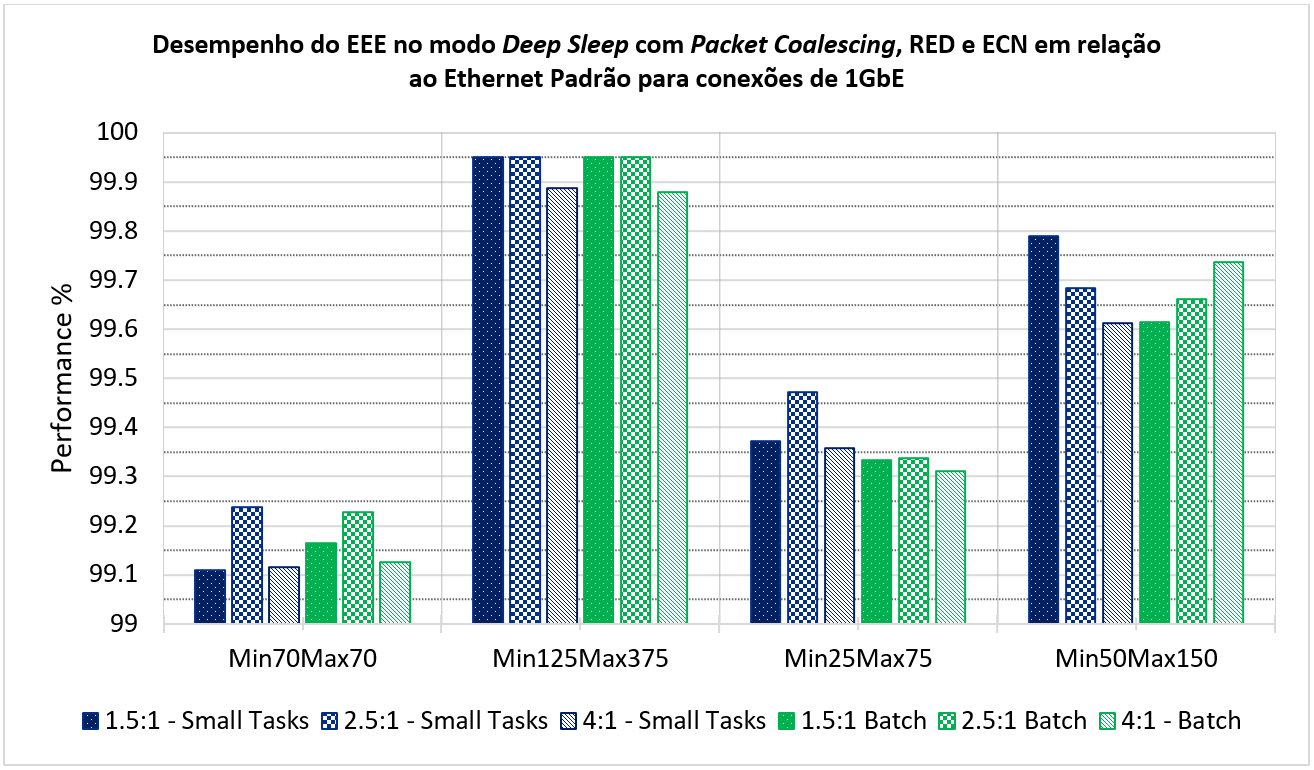
\includegraphics[width=8cm]{5-EEECoDelHadoop/PerfEEEDeepSleepPacoREDECN_1GbE.PNG}}\hfill
    \subfloat[\centering Desempenho do EEE no modo \emph{Deep Sleep} com \emph{Packet Coalescing}, RED e ECN em relação ao Ethernet Padrão para conexões de 10GbE
    \label{fig:PerfEEEDeepSleepPaCoREDECN10GbE}]{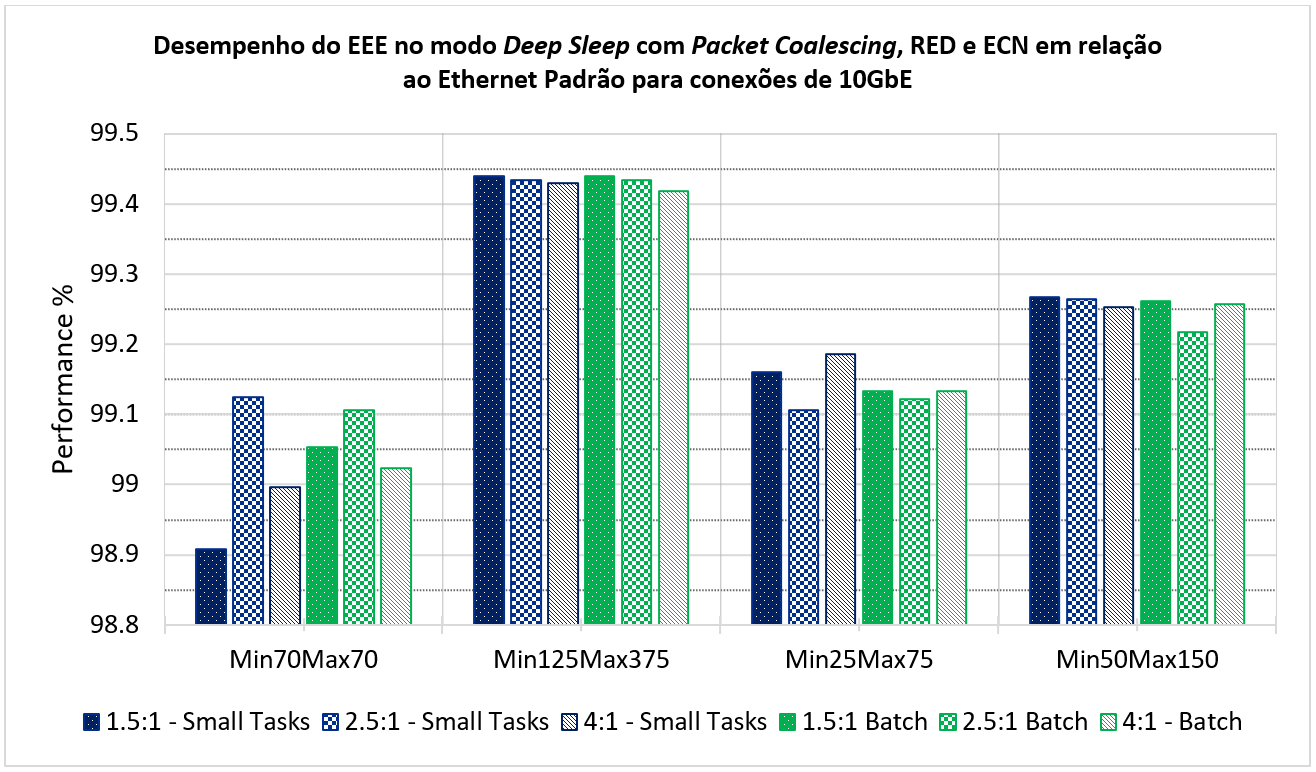
\includegraphics[width=8cm]{5-EEECoDelHadoop/PerfEEEDeepSleepPacoREDECN_10GbE.PNG}}
    
    \subfloat[\centering Desempenho do EEE no modo \emph{Deep Sleep} com \emph{Packet Coalescing}, RED e ECN em relação ao Ethernet Padrão para conexões de 25GbE \label{fig:PerfEEEDeepSleepPaCoREDECN25GbE}]{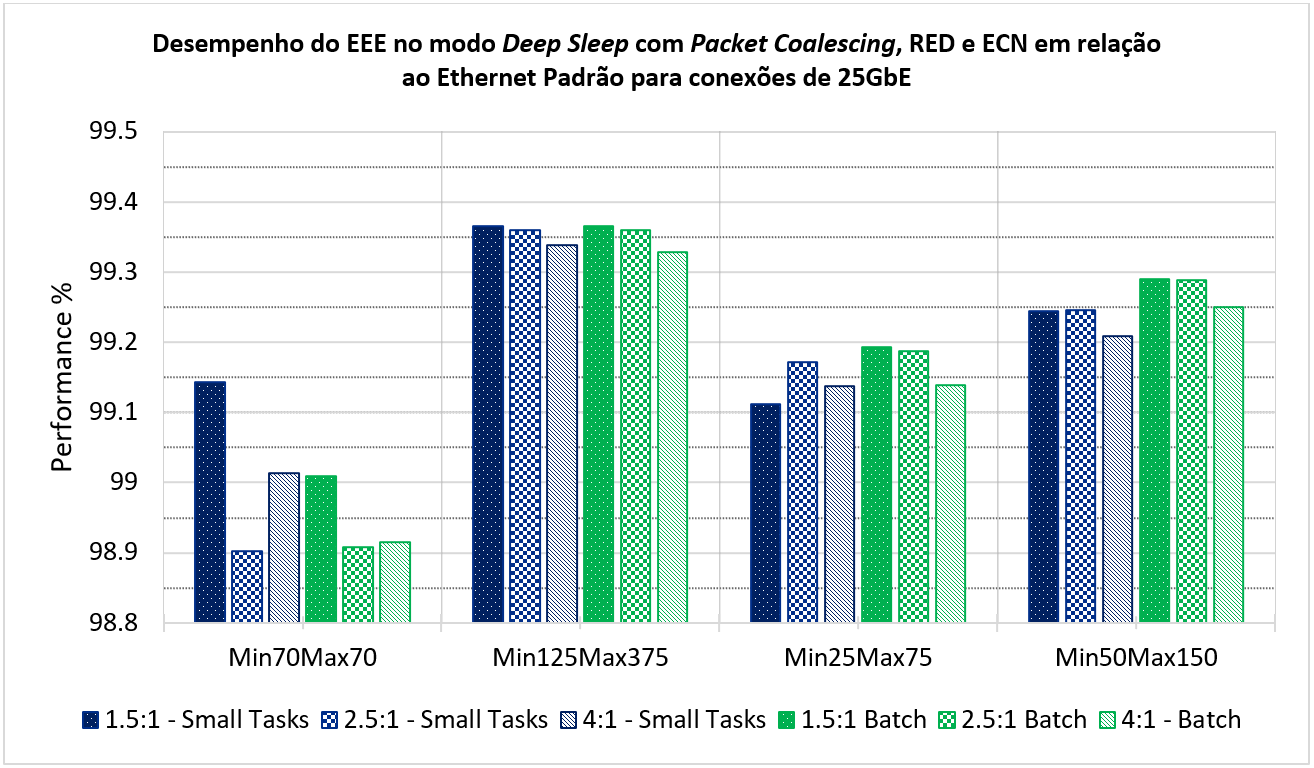
\includegraphics[width=8cm]{5-EEECoDelHadoop/PerfEEEDeepSleepPacoREDECN_25GbE.PNG}}\hfill
    \subfloat[\centering Desempenho do EEE no modo \emph{Deep Sleep} com \emph{Packet Coalescing}, RED e ECN em relação ao Ethernet Padrão para conexões de 40GbE
    \label{fig:PerfEEEDeepSleepPaCoREDECN40GbE}]{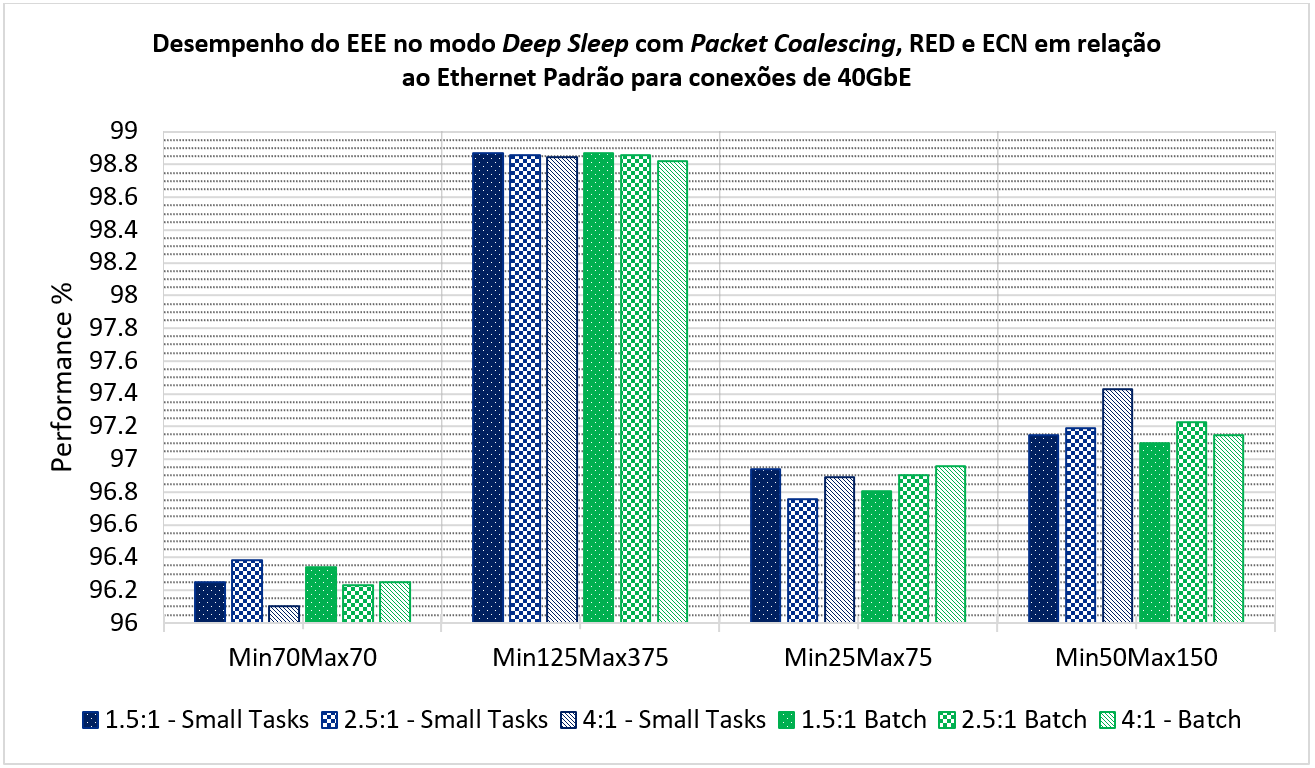
\includegraphics[width=8cm]{5-EEECoDelHadoop/PerfEEEDeepSleepPacoREDECN_40GbE.PNG}}    
    
    \subfloat[\centering Desempenho do EEE no modo \emph{Deep Sleep} com \emph{Packet Coalescing}, RED e ECN em relação ao Ethernet Padrão para conexões de 100GbE
    \label{fig:PerfEEEDeepSleepPaCoREDECN100GbE}]{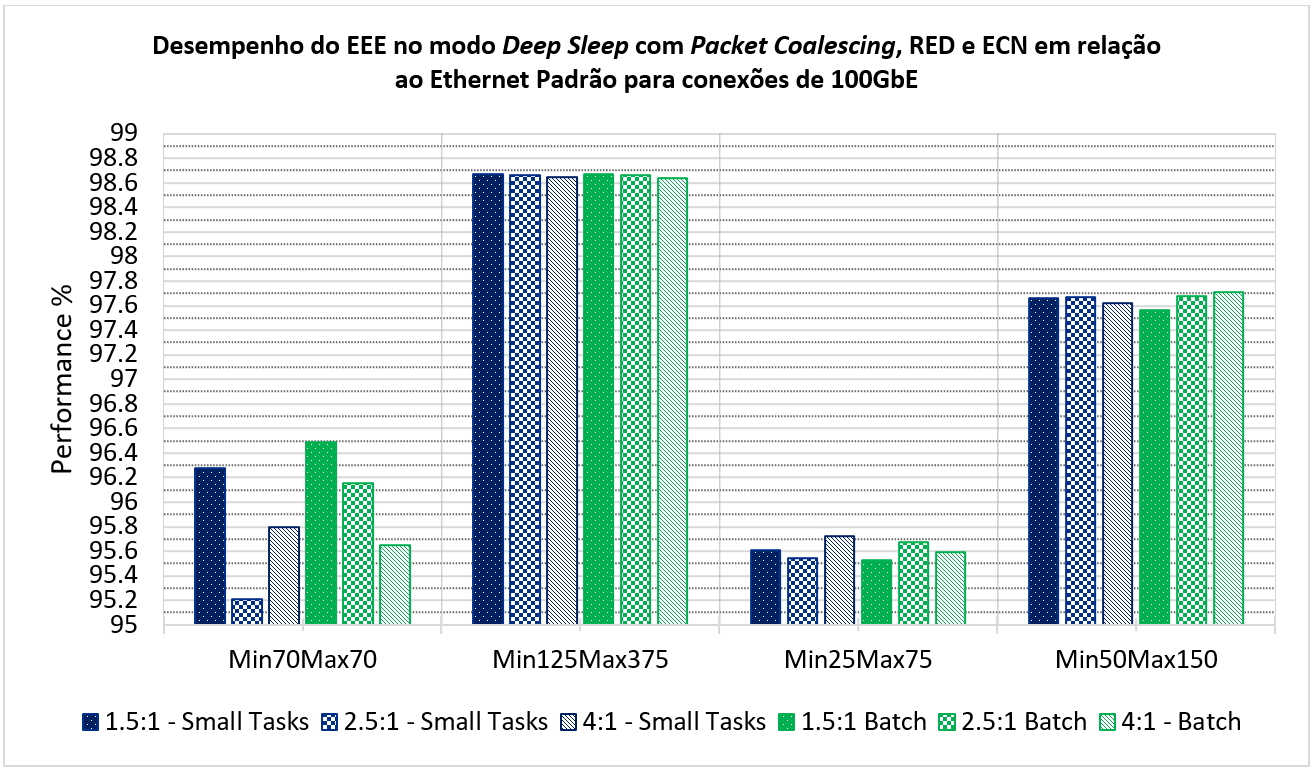
\includegraphics[width=8cm]{5-EEECoDelHadoop/PerfEEEDeepSleepPacoREDECN_100GbE.PNG}}\hfill
    \subfloat[\centering Desempenho do EEE no modo \emph{Deep Sleep} com \emph{Packet Coalescing}, RED e ECN em relação ao Ethernet Padrão para conexões de 400GbE
    \label{fig:PerfEEEDeepSleepPaCoREDECN400GbE}]{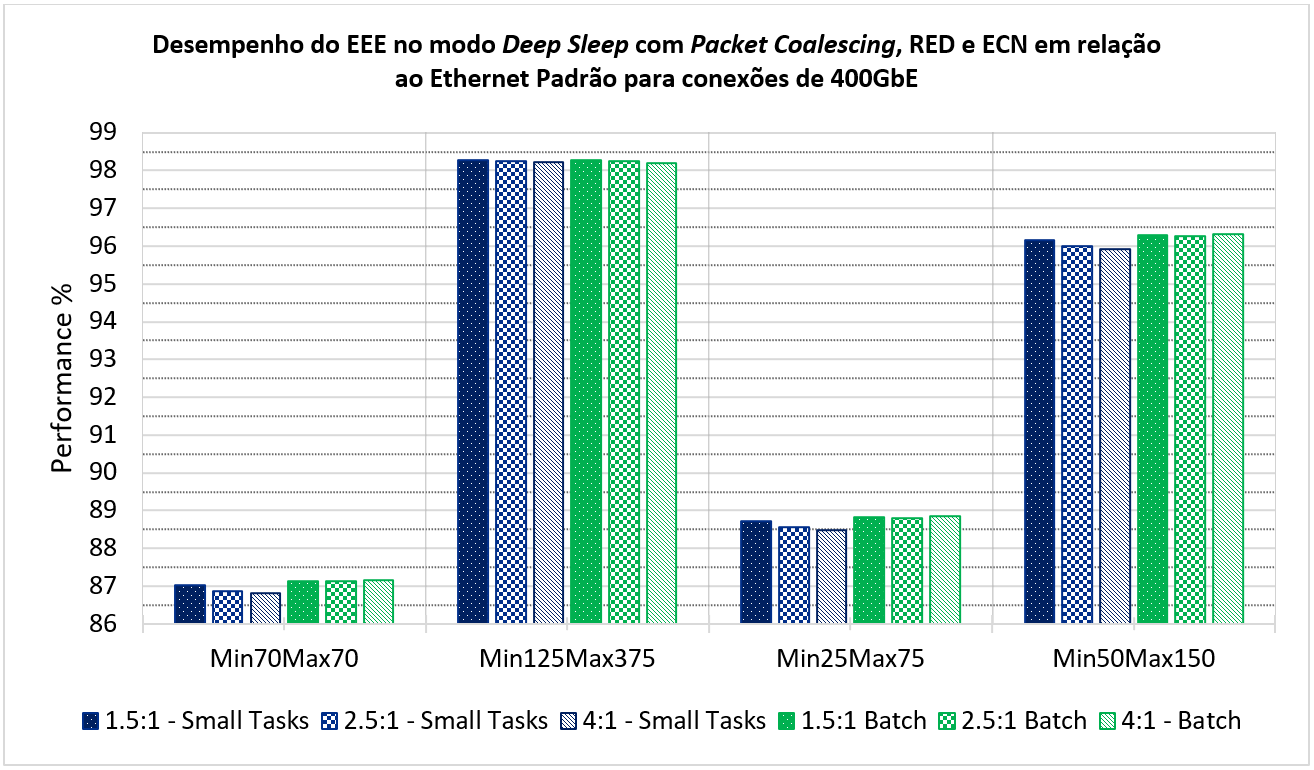
\includegraphics[width=8cm]{5-EEECoDelHadoop/PerfEEEDeepSleepPacoREDECN_400GbE.PNG}}       
    
    \caption{\centering Desempenho do EEE no modo \emph{Deep Sleep} com \emph{Packet Coalescing}, RED e ECN}
\end{figure}


\begin{figure}[p]
    \centering
    \label{fig:PerfEEEFastWakePaCoREDECN}
    
    \subfloat[\centering Desempenho do EEE no modo \emph{Fast Wake} com \emph{Packet Coalescing}, RED e ECN em relação ao Ethernet Padrão para conexões de 40GbE
    \label{fig:PerfEEEFastWakePaCoREDECN40GbE}]{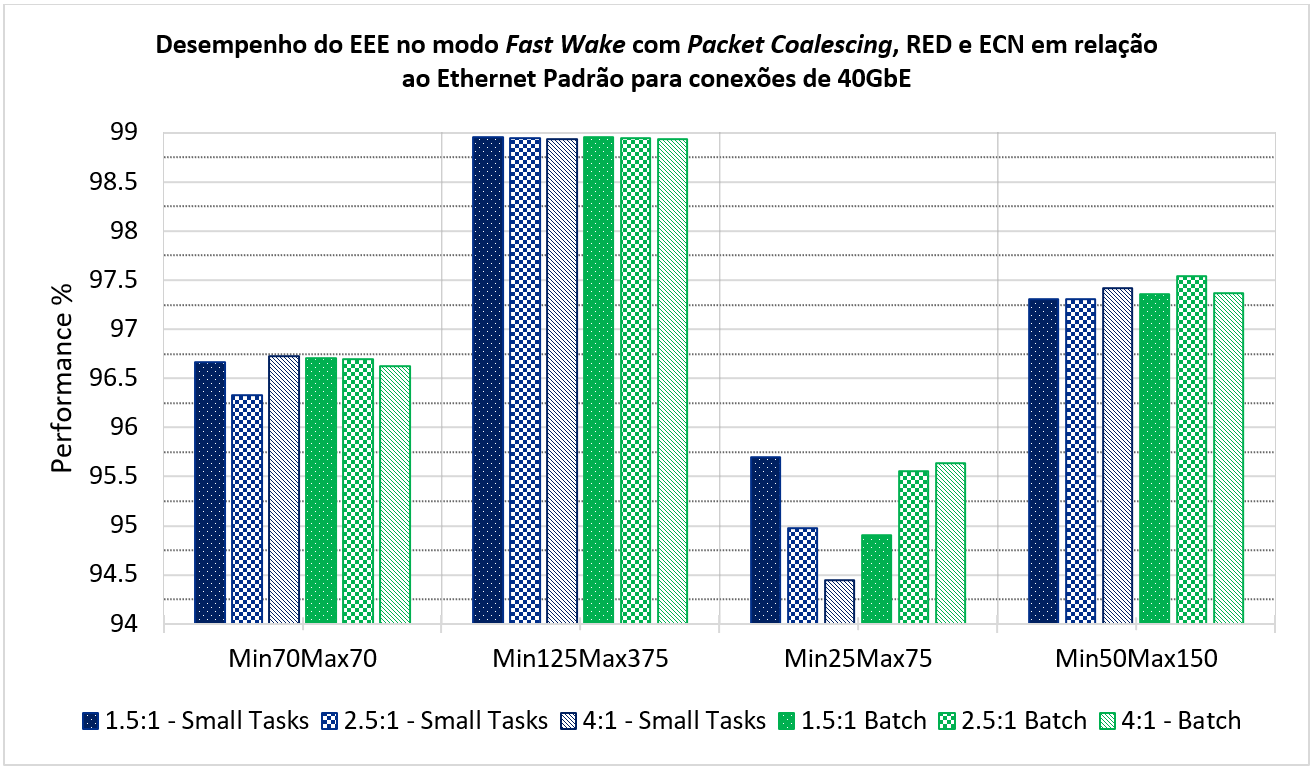
\includegraphics[width=8cm]{5-EEECoDelHadoop/PerfEEEFastWakePacoREDECN_40GbE.PNG}}\hfill
    \subfloat[\centering Desempenho do EEE no modo \emph{Fast Wake} com \emph{Packet Coalescing}, RED e ECN em relação ao Ethernet Padrão para conexões de 100GbE
    \label{fig:PerfEEEFastWakePaCoREDECN100GbE}]{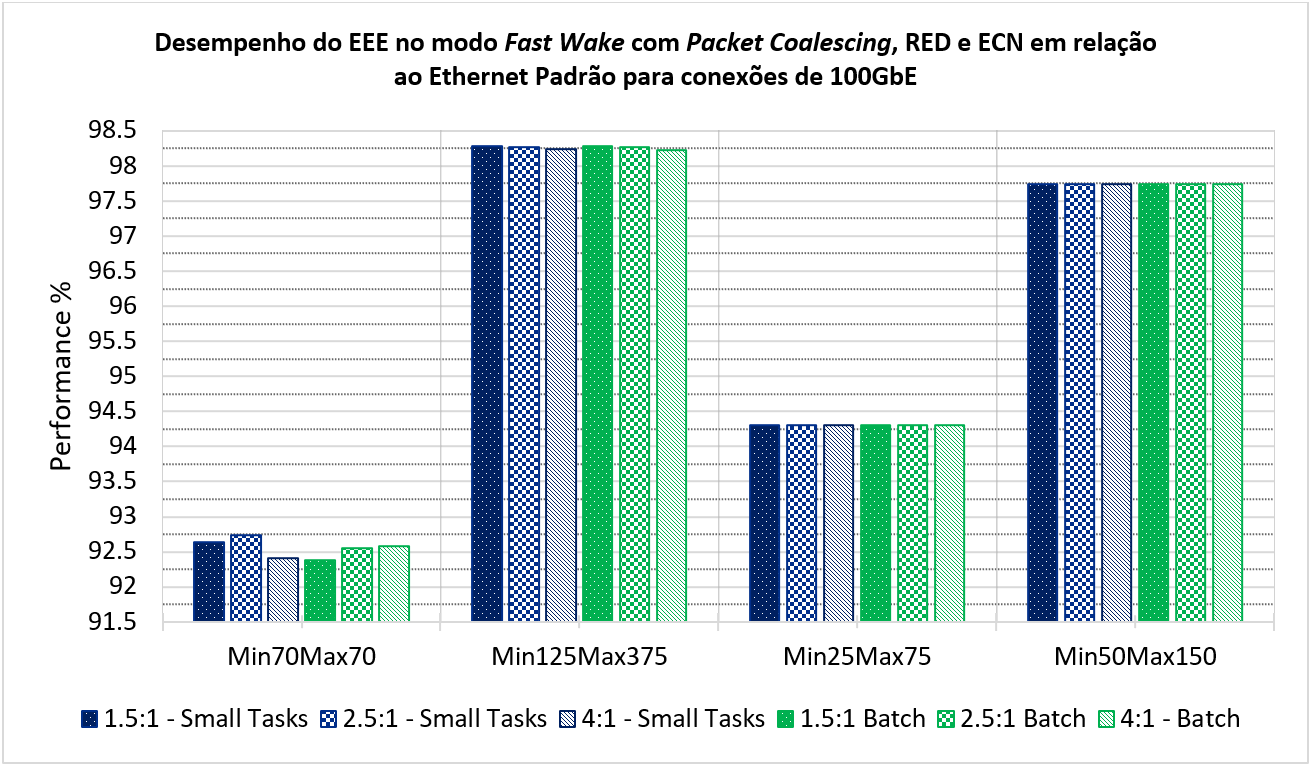
\includegraphics[width=8cm]{5-EEECoDelHadoop/PerfEEEFastWakePacoREDECN_100GbE.PNG}}
    
    \caption{\centering Desempenho do EEE no modo \emph{Fast Wake} com \emph{Packet Coalescing}, RED e ECN}
\end{figure}

Quanto aos links de 100GbE com \emph{Fast Wake}, o melhor parâmetro 125{$\mathit{Min}_\mathit{th}$}375{$\mathit{Max}_\mathit{th}$} aumentou o desempenho de 98.2\% para 98.26\%. Já em seu pior parâmetro 70{$\mathit{Min}_\mathit{th}$}70{$\mathit{Max}_\mathit{th}$}, degradou para 92.55\%.

Todos os resultados estão ilustrados de forma detalhada nas figuras 5.11 e 5.12. De forma geral o melhor parâmetro encontrado para o RED foi 125{$\mathit{Min}_\mathit{th}$}375{$\mathit{Max}_\mathit{th}$}, enquanto  70{$\mathit{Min}_\mathit{th}$}70{$\mathit{Max}_\mathit{th}$} e 25{$\mathit{Min}_\mathit{th}$}75{$\mathit{Max}_\mathit{th}$} degradaram consideravelmente a performance dos links.

\section{Comparação com o E-EON}

Esta seção abrange os conceitos do principal trabalho relacionado, o \emph{Energy-Efficient and Optimized Networks for Hadoop}, e uma comparação com os resultados obtidos durante nossa pesquisa. O E-EON \cite{silva2018eon} é um conjunto de técnicas que podem ser utilizadas para reduzir o consumo de energia e latência da rede, e melhorar a taxa de transferência do \emph{cluster} Hadoop. Além disso, tais técnicas não são exclusivas do Hadoop e podem ser aplicadas com benefícios semelhantes à qualquer outra carga de trabalho que se enquadre nas especificações do \emph{MapReduce}.

Este estudo foi o primeiro a avaliar o protocolo 802.2az \emph{Energy Efficient Ethernet} em \emph{clusters} Hadoop, e seus resultados demonstram que uma boa economia de energia pode ser obtida nas interconexões de folha (\emph{Leaf Interconnections}), mas no nível de agregação (\emph{Spines}) a coalescência de pacotes (\emph{Packet Coalescing}) é necessária para reduzir o consumo de energia a um nível próximo do ideal. Na mesma pesquisa, aconteceu a primeira análise do \emph{Active Queue Management} (AQM) e extensões de protocolo TCP que permitem o uso de ECN, como ECN autônomo e DCTCP. Os resultados apresentam uma redução da latência nas redes do Hadoop de 85\%, mantendo a taxa de transferência do \emph{cluster} em 95\% da linha de base. No entanto, não é uma tarefa fácil configurar tais filas.

Outra contribuição foi a compreensão do por que AQMs são tão difíceis de configurar em \emph{clusters} do Hadoop. Durante os testes foram identificados os motivos e caracterizado o padrão de tráfego que aumenta a latência e diminui a taxa de transferência de rede do \emph{cluster}, e, posteriormente, dadas sugestões de modificações de como as filas de comutação tratam os pacotes marcados com ECN. Uma redução da latência de rede e, em alguns casos, uma melhora do rendimento em 10\% foram alcançadas, e definido padrões de configurações.

Por fim, outros testes com conclusões residem na identificação das condições certas para combinar \emph{Energy Efficient Ethernet} e \emph{Packet Coalescing} com AQMs. A partir destes resultados é possível atingir um consumo de energia reduzido e redes de baixa latência.


\begin{figure}[!htb]
    \centering
    \label{fig:ComparaEEONEnergia}
    
    \subfloat[\centering Comparação dos resultados de consumo de energia entre Nossa Pesquisa e o E-EON em Conexões de 1GbE
    \label{fig:ComparaEEONEnergia1GbE}]{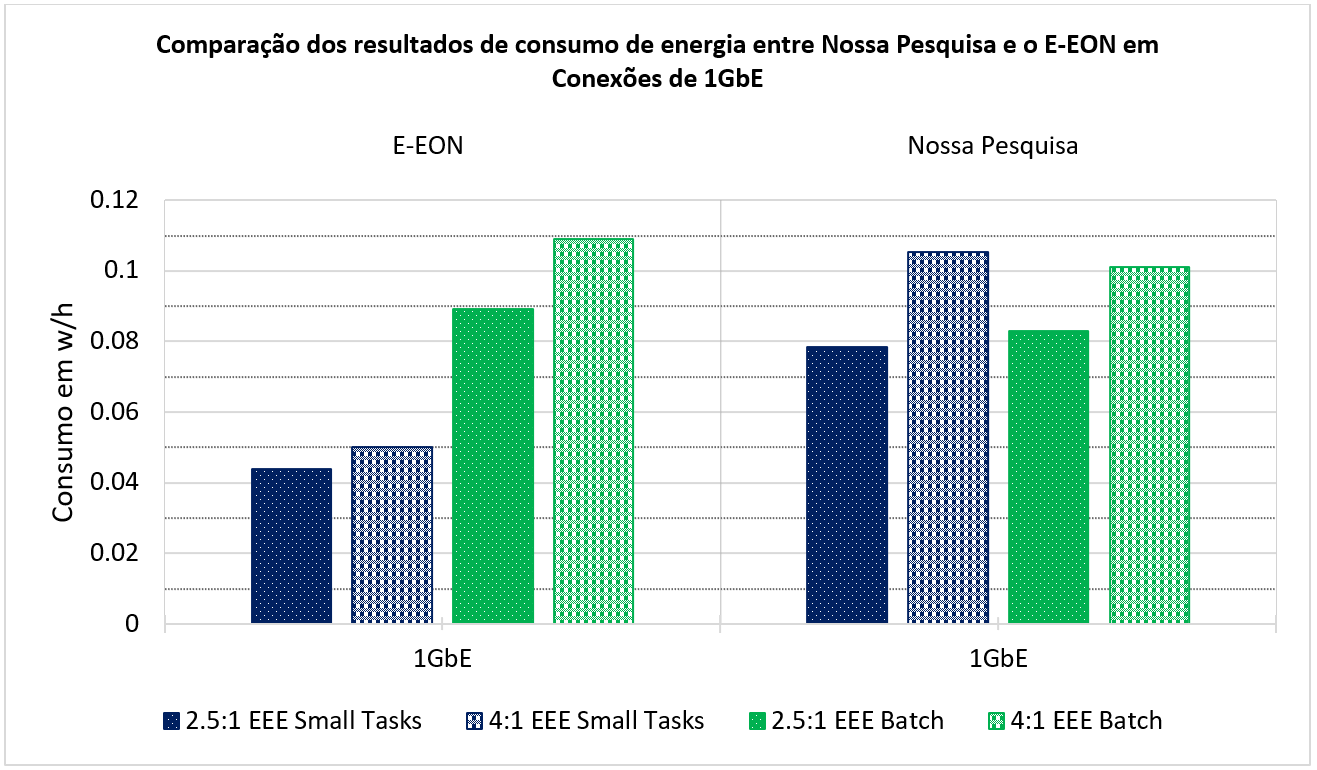
\includegraphics[width=8cm]{5-EEECoDelHadoop/Comparacao_1GbE_EEE_Energy_Consumption.PNG}}\hfill
    \subfloat[\centering Comparação dos resultados de consumo de energia entre Nossa Pesquisa e o E-EON em Conexões de 10GbE
    \label{fig:ComparaEEONEnergia10GbE}]{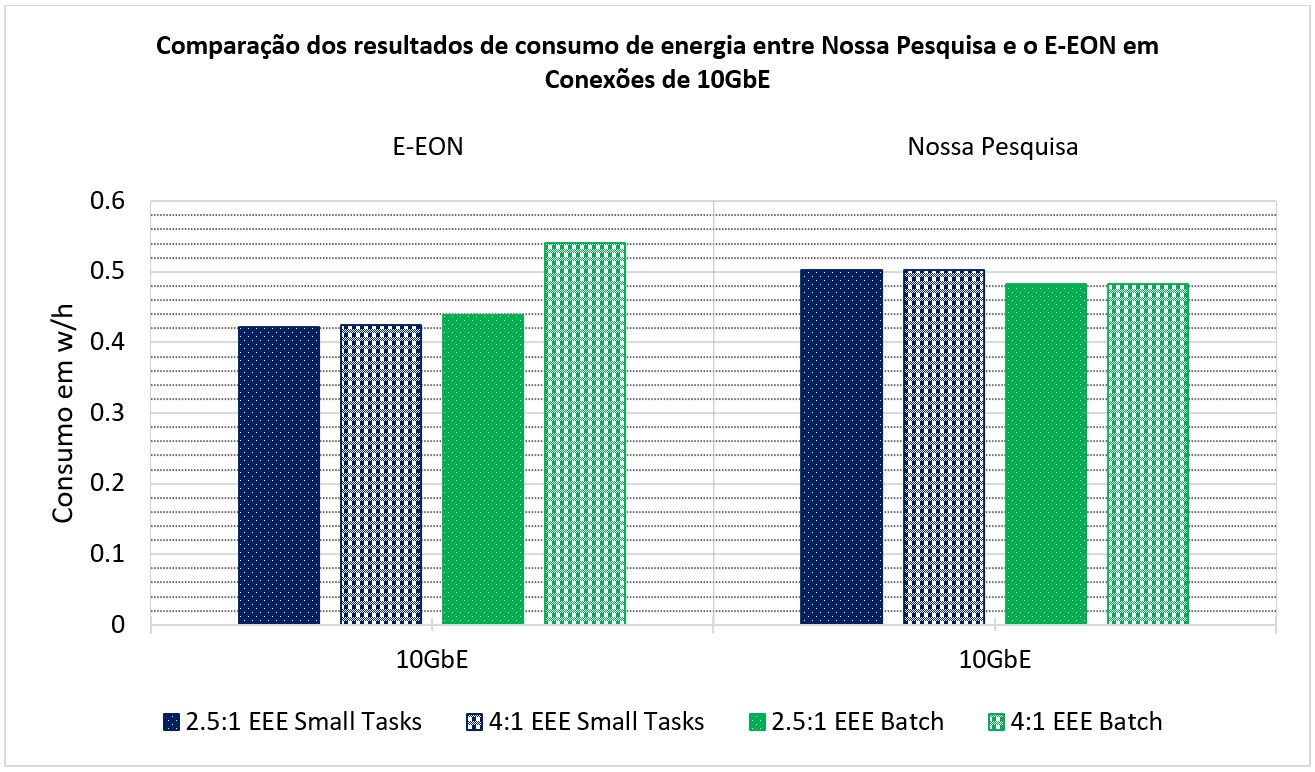
\includegraphics[width=8cm]{5-EEECoDelHadoop/Comparacao_10GbE_EEE_Energy_Consumption.PNG}}
    
    \caption{\centering Comparação dos resultados de consumo de energia entre Nossa Pesquisa e o E-EON}
\end{figure}

Os gráficos 5.13 e 5.14 expõem as leves diferenças entre os resultados de nossa pesquisa e o E-EON. Levando em consideração o desvio padrão, os resultados são tecnicamente iguais. Entretanto, a bibliografia disponível aponta que essas diferenças na verdade se devem a fatores como a arquitetura do Hadoop 1.x ser diferenciada do Hadoop 3.x com as introduções do YARN e EC \cite{white2009hadoop}; \cite{white2015hadoop}. Outra condição que pode contribuir é o fato de que o MRPerf \cite{wang2009using} utilizado nas simulações do E-EON possuí limitações para medir com precisão algumas etapas da estrutura do \emph{MapReduce}, especialmente nas fases de competição por recursos, tendo eficácia apenas na fase \emph{Shuffle} \cite{liu2013hsim}, enquanto o NetSLS \cite{wette2015extending} mede com precisão todas as etapas de uma aplicação, incluindo a alocação de recursos e inicialização dos \emph{Jobs} \cite{ApacheSLS}; \cite{wette2015extending}.

\begin{figure}[!htb]
    \centering
    \label{fig:ComparaEEONPerformance}
    
    \subfloat[\centering Comparação dos resultados de performance entre Nossa Pesquisa e o E-EON em Conexões de 1GbE
    \label{fig:ComparaEEONPerformance1GbE}]{\includegraphics[width=8cm]{5-EEECoDelHadoop/Comparacao_1GbE_EEE_Performance.PNG}}\hfill
    \subfloat[\centering Comparação dos resultados de performance entre Nossa Pesquisa e o E-EON em Conexões de 10GbE
    \label{fig:ComparaEEONPerformance10GbE}]{\includegraphics[width=8cm]{5-EEECoDelHadoop/Comparacao_10GbE_EEE_Performance.PNG}}
    
    \caption{\centering Comparação dos resultados de performance entre Nossa Pesquisa e o E-EON}
\end{figure}



\begin{figure}[!htb]
    \centering
    \label{fig:ComparaEEONEnergiaBestConfig}
    
    \subfloat[\centering Comparação dos resultados de consumo de energia com as melhores configurações entre Nossa Pesquisa e o E-EON em Conexões de 1GbE
    \label{fig:ComparaEEONEnergia1GbEBestConfig}]{\includegraphics[width=8cm]{5-EEECoDelHadoop/Comparacao_1GbE_EEE_Energy_Consumption_BestConfig.PNG}}\hfill
    \subfloat[\centering Comparação dos resultados de consumo de energia com as melhores configurações entre Nossa Pesquisa e o E-EON em Conexões de 10GbE
    \label{fig:ComparaEEONEnergia10GbEBestConfig}]{\includegraphics[width=8cm]{5-EEECoDelHadoop/Comparacao_10GbE_EEE_Energy_Consumption_BestConfig.PNG}}
    
    \caption{\centering Comparação dos resultados de consumo de energia com as melhores configurações entre Nossa Pesquisa e o E-EON}
\end{figure}



\begin{figure}[!htb]
    \centering
    \label{fig:ComparaEEONPerformanceBestConfig}
    
    \subfloat[\centering Comparação dos resultados de performance com as melhores configurações entre Nossa Pesquisa e o E-EON em Conexões de 1GbE
    \label{fig:ComparaEEONPerformance1GbEBestConfig}]{\includegraphics[width=8cm]{5-EEECoDelHadoop/Comparacao_1GbE_EEE_Energy_Consumption_BestConfig.PNG}}\hfill
    \subfloat[\centering Comparação dos resultados de performance com as melhores configurações entre Nossa Pesquisa e o E-EON em Conexões de 10GbE
    \label{fig:ComparaEEONPerformance10GbEBestConfig}]{\includegraphics[width=8cm]{5-EEECoDelHadoop/Comparacao_10GbE_EEE_Energy_Consumption_BestConfig.PNG}}
    
    \caption{\centering Comparação dos resultados de performance com as melhores configurações entre Nossa Pesquisa e o E-EON}
\end{figure}

As figuras 5.15 e 5.16 mostram os resultados de economia de energia e performance para o E-EON e também para nossa pesquisa. De modo geral, em ambos os trabalhos, as configurações do \emph{Packet Coalescing} usando o parâmetro 120$\mu$s100, AQM \emph{Random Early Detection} no modo \emph{Instant Queue Length} com parâmetro 125{$\mathit{Min}_\mathit{th}$}375{$\mathit{Max}_\mathit{th}$} e \emph{Explicit Congestion Notification} no modo \emph{Default} performaram melhor, oferecendo uma ótima economia de energia com uma perda mínima de desempenho.

Durante nossos testes não levamos em conta o DCTCP, uma vez que não houve resultados satisfatórios em \cite{silva2018eon}. Por outro lado, para o EEE testamos os dois modos disponíveis, o \emph{Deep Sleep} e o \emph{Fast Wake}, enquanto no E-EON foi levado em conta apenas o modo \emph{Deep Sleep}. Além da pesquisa feita no E-EON para conexões de 1GbE e 10GbE fomos adiante realizando simulações e oferecendo resultados de economia de energia e performance com o EEE habilitado para conexões de 25GbE, 40GbE, 100GbE e 400GbE. Em contrapartida, o E-EON procurou aumentar a largura de banda do \emph{cluster} e reduzir a latência em conexões Ethernet comuns (sem o EEE), mas este não era o foco de nossa pesquisa.


\section{Considerações Finais}

Neste capítulo foram apresentados estudos experimentais (simulações) com o objetivo de reduzir ainda mais o consumo de energia aliando o \emph{Energy Efficient Ethernet} ao \emph{Packet Coalescing}. Posteriormente aplicamos \emph{Active Queue Managements} como \emph{Controlled Delay} e \emph{Random Early Detection} com \emph{Explicit Congestion Notification} para recuperar a performance degradada pelo EEE e \emph{Packet Coalescing}, obtendo assim redes com baixo consumo de energia e desempenho próximo ao Ethernet Padrão.

Durante nossos experimentos encontramos resultados que demonstram que quando configurado corretamente, com o melhor parâmetro 120$\mu$s100, o \emph{Packet Coalescing} juntamente ao EEE proporciona uma redução do consumo de energia até 45\% maior em relação ao EEE padrão.

Ao procurarmos por soluções de AQMs para reduzir a perda de desempenho apresentada pelo EEE e EEE com \emph{Packet Coalescing}, o RED com a configuração 125{$\mathit{Min}_\mathit{th}$}375{$\mathit{Max}_\mathit{th}$} demonstrou ser 65\% mais eficiente que o CoDel com todas as suas configurações 500$\mu$s20ms, 300$\mu$s0.75$\mu$s, 400$\mu$s1ms e 800$\mu$s1.5ms. Uma explicação para tal diferença é que o RED usando o modo IQL (\emph{Instant Queue Length}) acaba sendo mais responsivo do que o cálculo dinâmico realizado pelo CoDel \cite{silva2018eon}. Sendo assim, segue um sumário da melhor combinação que proporciona um \textbf{balanceamento entre economia de energia e desempenho} encontrada para cada conexão:

\begin{itemize}

\item \textbf{1GbE}: \emph{Energy Efficient Ethernet} no modo \emph{Deep Sleep}. Esta configuração proporciona uma economia de energia de 83.89\% com uma perda de desempenho de apenas 0.217\% em relação ao Ethernet Padrão;


\item \textbf{10GbE}: \emph{Energy Efficient Ethernet} no modo \emph{Deep Sleep}, com \emph{Packet Coalescing} usando o parâmetro 120$\mu$s100, AQM \emph{Random Early Detection} no modo \emph{Instant Queue Length} com parâmetro 125{$\mathit{Min}_\mathit{th}$}375{$\mathit{Max}_\mathit{th}$} e \emph{Explicit Congestion Notification} no modo \emph{Default}. Esta configuração proporciona uma economia de energia de 88.4\% com uma perda de desempenho de 0.57\% em relação ao Ethernet Padrão;


\item \textbf{25GbE}: \emph{Energy Efficient Ethernet} no modo \emph{Deep Sleep}, com \emph{Packet Coalescing} usando o parâmetro 120$\mu$s100, AQM \emph{Random Early Detection} no modo \emph{Instant Queue Length} com parâmetro 125{$\mathit{Min}_\mathit{th}$}375{$\mathit{Max}_\mathit{th}$} e \emph{Explicit Congestion Notification} no modo \emph{Default}. Esta configuração proporciona uma economia de energia de 86.88\% com uma perda de desempenho de 0.65\% em relação ao Ethernet Padrão;


\item \textbf{40GbE}: \emph{Energy Efficient Ethernet} no modo \emph{Deep Sleep}, com \emph{Packet Coalescing} usando o parâmetro 120$\mu$s100, AQM \emph{Random Early Detection} no modo \emph{Instant Queue Length} com parâmetro 125{$\mathit{Min}_\mathit{th}$}375{$\mathit{Max}_\mathit{th}$} e \emph{Explicit Congestion Notification} no modo \emph{Default}. Esta configuração proporciona uma economia de energia de 87.03\% com uma perda de desempenho de 1.15\% em relação ao Ethernet Padrão;



\item \textbf{100GbE}: \emph{Energy Efficient Ethernet} no modo \emph{Deep Sleep}, com \emph{Packet Coalescing} usando o parâmetro 120$\mu$s100, AQM \emph{Random Early Detection} no modo \emph{Instant Queue Length} com parâmetro 125{$\mathit{Min}_\mathit{th}$}375{$\mathit{Max}_\mathit{th}$} e \emph{Explicit Congestion Notification} no modo \emph{Default}. Esta configuração proporciona uma economia de energia de 84.64\% com uma perda de desempenho de 1.342\% em relação ao Ethernet Padrão;



\item \textbf{400GbE}: \emph{Energy Efficient Ethernet} no modo \emph{Deep Sleep}, com \emph{Packet Coalescing} usando o parâmetro 120$\mu$s100, AQM \emph{Random Early Detection} no modo \emph{Instant Queue Length} com parâmetro 125{$\mathit{Min}_\mathit{th}$}375{$\mathit{Max}_\mathit{th}$} e \emph{Explicit Congestion Notification} no modo \emph{Default}. Esta configuração proporciona uma economia de energia de 74.73\% com uma perda de desempenho de 1.765\% em relação ao Ethernet Padrão;


\end{itemize}

No modo \emph{Fast Wake} do \emph{Energy Efficient Ethernet} os melhores resultados que fornecem balanceamento entre economia de energia e desempenho foram encontrados ao utilizar apenas a tecnologia do \emph{Packet Coalescing} com o parâmetro 120$\mu$s100. Esta configuração proporciona uma economia de energia nos links de 40GbE e 100GbE de 59.7\% e 59.63\% com uma perda de desempenho de 1.11\% e 1.72\% em relação ao Ethernet Padrão respectivamente.

Por fim, avaliamos assim como \cite{herreria2017optimizing} que o uso do modo \emph{Fast Wake} do EEE se torna útil para administradores com baixo conhecimento em infraestrutura, pois de modo geral, proporciona um desempenho similar ao EEE no modo \emph{Deep Sleep} configurado com \emph{Packet Coalescing}, RED e ECN, porém, com um consumo de energia maior.
